\documentclass{uai2023} % for initial submission
% \documentclass[accepted]{uai2023} % after acceptance, for a revised
                                    % version; also before submission to
                                    % see how the non-anonymous paper
                                    % would look like
%% There is a class option to choose the math font
% \documentclass[mathfont=ptmx]{uai2023} % ptmx math instead of Computer
                                         % Modern (has noticable issues)
% \documentclass[mathfont=newtx]{uai2023} % newtx fonts (improves upon
                                          % ptmx; less tested, no support)
% NOTE: Only keep *one* line above as appropriate, as it will be replaced
%       automatically for papers to be published. Do not make any other
%       change above this note for an accepted version.

%% Choose your variant of English; be consistent
\usepackage[american]{babel}
% \usepackage[british]{babel}

%% Some suggested packages, as needed:
\usepackage{natbib} % has a nice set of citation styles and commands
    \bibliographystyle{plainnat}
    \renewcommand{\bibsection}{\subsubsection*{References}}
% \usepackage{mathtools} % amsmath with fixes and additions
% \usepackage{siunitx} % for proper typesetting of numbers and units
\usepackage{booktabs} % commands to create good-looking tables
% \usepackage{tikz} % nice language for creating drawings and diagrams

\input{confidence-preamble}
% \addbibresource{conf.bib}

%% Provided macros
% \smaller: Because the class footnote size is essentially LaTeX's \small,
%           redefining \footnotesize, we provide the original \footnotesize
%           using this macro.
%           (Use only sparingly, e.g., in drawings, as it is quite small.)

%% additional macros
\newcommand{\ext}[1]{\overline #1} %  measures over phi
\newcommand{\Unif}{\mathrm{Unif}}

\newcommand\cofunc{commitment function}
\newcommand\confdom{\mathdcal C}
\newcommand\ZO{\mathrm{ZO}}
% \def\ZO{[0,1]}
\newcommand\Rplus{\mathbb R_+}
\newcommand\X{\mathcal X}

% \let\oldTheta\Theta
% \renewcommand\Theta{\mathdcal{\Theta}}

% \title{Measures of Confidence}
\title{%
    % Updating with Confidence
    Updating with Confidence
}

% The standard author block has changed for UAI 2022 to provide
% more space for long author lists and allow for complex affiliations
%
% All author information is authomatically removed by the class for the
% anonymous submission version of your paper, so you can already add your
% information below.

% Add authors
\author[1]{\href{mailto:<oer5@cornell.edu>?Subject=confidence-paper}{Oliver E Richardson}{}}
\author[1]{Joseph Y Halpern}
% Add affiliations after the authors
\affil[1]{%
    Computer Science Dept.\\
    Cornell University\\
    Ithaca, New York, USA
}

\begin{document}
\maketitle

\begin{abstract}
We introduce a new notion of confidence, which arises when learning or updating beliefs.
\end{abstract}

\section{Introduction}\label{sec:intro}
\def\stmt{$A$}
% \def\stmt{$\phi$}

% The ability articulate a \emph{degree of confidence} is an important aspect of knowledge representation.
The ability to articulate a \emph{degree of confidence} 
% (or the opposite: a degree of uncertainty)
is a critical aspect of representing knowledge.
% is an important aspect of representing knowledge.
	% Subpoint: it helps avoid a brittleness of always beliving things
	% Subpoint: Protects against overconfidence.
There are 
% Correspondingly, there are
many well-established ways to quantify (un)certinaty \parencite[\S2]{halpern2017reasoning},
	% probability chief among them.	
	and chief among them is probability.
	% perhaps most common is to use probabilities.
% Indeed, many people use ``confidence'' as a synonym for probability.
% Indeed, ``confidence'' is often used as a synonym for probability. 
% Indeed, ``high confidence'' and ``high probability'' are often used interchangably. 
% Indeed, ``confidence'' and 
% In our view, this practice
% Although this use of the word is perfectly functional, it seems to have shadowed another conception of confidence---one that is fundementally different, if at first sublty so.
% However, this practice shadows
% However, this practice seems to have shadowed 
% However, there is also another conception
% However, there
% However, there is also another conception 
% 	of confidence---one that is fundementally different, if at first subtly so.
% Although there is nothing wrong with this, 
% which seems have been shadowed by the enormous success of probability---one that is fundementally different, if at first subtly so.
% which seems to have been shadowed by the enormous success of probability---a concept that is fundementally different, if at first subtly so.
% This paper develops that notion 
% However, there is also another conception of confidence---one that complements traditional representations of uncertainty, and is fundementally different in nature. 
% In our view, however, there is also another conception of confidence:
% 	% one that complements traditional representations of uncertainty, and is fundementally different in nature. 
% 	one that complements traditional representations of uncertainty (such as probability), and is fundementally different in nature. 
% In our view, however, there is also another conception of confidence
% While ``confidence'' admits a coherent probabilistic reading,
While ``confidence'' can be coherently read in probabilistic terms,
	such usage may shadow another important concept.
This paper details a different conception that arises when updating beliefs. 
% This paper describes a very different conception of confidence that arises when updating beliefs. 
	% one that complements traditional representations of uncertainty, and is fundementally different in nature. 
% This alternate conception of confidence, which is the focus of the present paper,
% This alternate conception
As we shall see, this notion of confidence
% can be used alongside 
complements traditional representations of uncertainty (such as probability), 
% but is fundementally different in nature. 
and moreover unifies several different concepts
across AI.
% ranging from traditional notions of confidence like inverse variance, and Shafer's weight of evidence, to notions in ML and optimization: learning rates and objective strengths. 
% We develop this notion 


% For us, confidence is a measure of trust (in incoming information), rather than of likelihood (of hypothetical information). 
For us, confidence (in an input $\phi$) is a measure of \emph{trust}, rather than of likelihood; it quantifies seriously to take $\phi$ in updating one's beliefs.
% Like probability, confidence lies on a continuum between two extremes---but they have different meanings.
% To see how the two notions diverge, imagine learning something surprising from a trusted source; that piece of information has high confidence but low probability.
% While confidence and probability are often 
Likelihood and trust often tightly coupled, but they are different.
For example, we might trust a surprising piece of information despite thinking it unlikely.
%
Of course, after updating, we would find that same information likely (precisely because we took it seriously in the update).
%
Thus, high confidence implies high posterior likelihood, making it easy to confuse the two.
The converse, however, is not true:
% information from an untrusted source, but that you happen to already believe, should be ascribed high (prior and posterior) likelihood, but low confidence.
% to information from an untrusted source that we happen to already believe, we should ascribe high (prior and posterior) likelihood but low confidence.
we should ascribe high (prior \emph{and} posterior) likelihood, but low confidence, to information from an untrusted source which we happen to believe already.
% we should ascribe high (prior and posterior) likelihood but low confidence information from an untrusted source, but that you happen to already believe, should be ascribed high (prior and posterior) likelihood, but low confidence.

% in an updating context: it's how seriously you take an input
% What we have in mind applies in an updating or learning setting. 
% We take confidence (in an input $\phi$) to be a measure of how seriously we take $\phi$ in updating our beliefs.
% Like probability, confidence lies in continuum between two extremes, but it ranges from untrusted to trusted, rather than from unlikely to likely.
% More concretely, confidence interpolates between prior beliefs and the beliefs one would obtain by fully incorporating $\phi$, so as to obtain posterior beliefs somewhere in between. 
More concretely, confidence interpolates between prior beliefs and those obtained by fully trusting $\phi$, so as to obtain posterior beliefs somewhere in between. 
Consequently, the notion is heavily dependent on the geometry of beliefs.
% This already suffices to characterize our simplest running example:
To take a simple example,
if our prior belief is a probability measure $p$ over a finite set $X$, then to update on event $A$ with confidence $\chi \in [0,1]$ might be to arrive at the posterior belief $p'(X) = (1-\chi) p(X) + (\chi)\, p(X|A)$. 
% In this case, $\chi$ can be viewed as a ``fraction of incorporation''.
Note that 
an update with no confidence ($\chi{\,=\,}0$) ignores new information (since $p' \!=\! p$),
while a
% more customary
full confidence update ($\chi{\,=\,}1$) takes it as seriously as possible,
% (since then $p'(A) \!=\! 1$).  
since afterwards $p'(A) \!=\! 1$ and there is no way to further incorporate $A$.
%
%
% It is less clear that the intermediate points are the ``right'' ones, or that this 
% is the ``appropriate'' parameterization of the path
The particular choice of path, as well as its parameterization,
% are arguably natural consequences of the geometry of probability measures lying .
are open for debate, but are natural consequences of the geometry when we think of probabilities as points in a simplex.
%
In this context, 
% full confidence updates are customary, and
the confidence $\chi \in [0,1]$ has a clear interpretation as the ``fraction of the way towards full incorporation'',
% In other cases, however, 
% This is not always true.
but in others,
% it may not be clear what an intermediate number (say, $\chi=0.7$) means.
% it is less clear what such a number (say, $\chi=0.7$) means.
% it is still important to articulate confidence, but 
it may be 
%it is
less clear what a number on this scale (say, $\chi{=}0.7$) means.
% there is still a natural path from distrust to complete trust that is parameterized differently.
% it is less clear how to interpret such a number (say, $\chi=0.7$).
% In other cases, there are other more natural ways to articulate one's confidence.
% there are other, more natural ways to measure confidence.

% The confidence domain $[0,1]$ 
% In general, it is not clear what a confidence $\chi \in [0,1]$ means, and the scale starts to be less useful.
% In other cases, however, it is not so clear what it means to go, say, ``70\% of the way'' to fully incorparting information. 
% We still have a sensible notion of confidence in these cases, . 
% We now describe such an example.
% One such example is training a neural network. 
Consider a neural network, whose ``belief'' state is a setting of weights.
	% which are updated when given a training point.
% As it sees each training point, it updates its weights. 
% Modern learning algorithms do not take any individual point too seriously; each training point $x$ changes the weights incrementally, and alone may not even be enough for the network to classify that point correctly.
Modern learning algorithms (like gradient descent) make small incremental changes to the weights, and updating with a training example $x$ does not guarantee that the resulting network handles $x$ correctly. 
% In other words, the algorithm does not take any individual point too seriously.
In other words, such algorithms 
(in contrast to their historical counterparts \parencite{conjunctions}) 
do not take any one encounter with a training example too seriously.
% So, in contrast with conditioning, there is a significant difference betwen cycling through the training data once, and doing so many times.
This distrust of any individual observation is arguably what makes the training process so robust to noisy and conflicting observations.
\commentout{
	As a result,
	there is a significant difference between going through the training data once
	 % (a single epoch)
	\unskip, and doing so many times.}
Nevertheless, the weights do eventually converge if we repeatedly train on $x$, 
% which is a natural notion of 
% % ``fully incorporating $x$''---%
% full incorporation---%
an extreme action that is only appropriate if we trust $x$ completely.
% At the other extreme, if we had no trust in $x$, we could ignore it leaving our weights unchanged. 
% In this context, 
% Once again we have two extremes:
% Depending on our confidence, 
% How we ought to treat $x$ 
% What we ought to do depends on our confidence.
% At one extreme, we have no trust in $x$ and should ignore it, leaving weights unchanged; at the other, we trust $x$ completely, we should adopt the weights that arise in the limit of infinite training. 
% Moreover, this sequence of incremental updates (roughly) describes a path between the two extremes.%
Moreover, this sequence of incremental updates describes a path, from the opposite, low-confidence extreme of ignoring $x$.%
	\footnote{This path can be made into a continuous path by interpolating with a line segment, and made smooth in the limit of small step sizes; we will deal with both constructions in \cref{sec:project-additive}.}
Note that the relevant geometry here is not just the geometry of the weight space, but also that induced by the architecture and the loss function.
% As we will see in \cref{sec:loss-repr}, such 
% We have now seen a new way of quantifying confidence: the number of training iterations.
% The number of training iterations a different way of quantifying confidence.  
It is not so clear that a fraction of the way to completion (say 0.7) is as meaningful here as it was before (and it would be difficult to recognize that point in any case),
but we now have a different way to quantify confidence: the number of training iterations. 
% It turns out that in general, there are close relationships 

While there are some good reasons to prefer the first approach, 
the second one is more general. 
We can treat the example in this way: once we fix a ``unit confidence'', say $\chi=0.01$, a sequence of $n$ unit updates is equivalent to a single one of confidence $\chi= 1-(0.99)^n$. 
This general idea can be cleaned by appeal to differential geometry.
Specifically, we can take a limit

Moreover, in the case where belief states are Dempster-Shafer belief functions, 
and inputs are simple support functions, this measure of confidence is what Shafer calls the \emph{weight of evidence} \parencite{shafer1976mathematical}.

the updating process can be written as a vector field.




% natural measure of confidence that works in all cases,
% which 
% It turns out that there is a natural way of measuring confidence in all cases of interest, based on differential geometry of belief space. 
% Furthermore, in the case where belief states are Dempster-Shafer belief functions, 
% and inputs are simple support functions, this measure of confidence is what Shafer calls the ``weight of evidence''.
%% TODO: Shafer


%%%%% PARAGRAPH ON MANY DIFFERENT VIEWPOINTS
% Linear interpolation, however, is just the tip of 
% At the heart of our paper is a hierarchy 



\begin{figure}
\centering
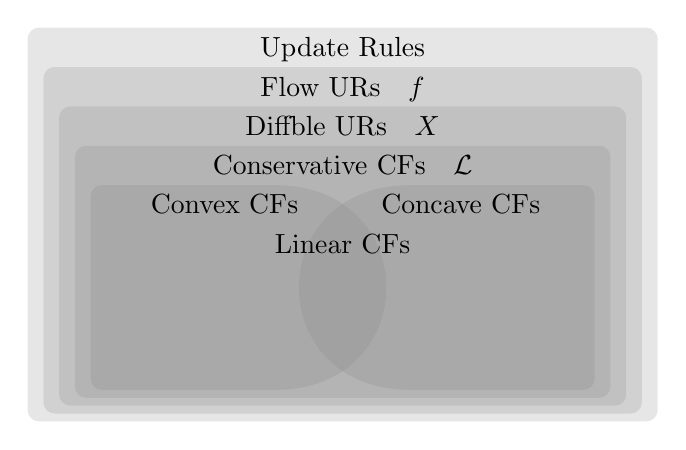
\begin{tikzpicture}
	\begin{scope}[fill=gray,fill opacity=0.2,rounded corners=4px]
		\fill (0,0) rectangle (8,5); % URs (Full Updates)
		\fill[] (0.2,0.1) rectangle (7.8,4.5); % Flow URs (Flows)
		\fill[] (0.4,0.2) rectangle (7.6,4.0); % Diffble URs (Vec Field)
		\fill[] (0.6,0.3) rectangle (7.4,3.5); % Conservative URs 
		\fill (0.8,0.4) -- (0.8, 3.0) -- (3, 3.0)
		 	to[out=0,in=0,looseness=2] (3,0.4) --cycle; % CONVEX
		\fill (7.2,0.4) -- (7.2, 3.0) -- (5, 3.0)
		 	to[out=180,in=180,looseness=2] (5,0.4) --cycle; % CONCAVE
	\end{scope}
	\begin{scope}[anchor=north]
		\node at (4.0, 5.0) {Update Rules};
		\node at (4.0, 4.5) {Flow URs~~~$f$};
		\node at (4.0, 4.0) {Diffble URs~~~$X$};
		% \node at (4.0, 3.5) {Conservative CFs~~~$\mathcal L$};
		\node at (4.0, 3.5) {Conservative CFs~~~$\mathcal L$};
		\node at (2.5, 3.0) {Convex CFs};
		\node at (4.0, 2.5) {Linear CFs};
		\node at (5.5, 3.0) {Concave CFs};
	\end{scope}
\end{tikzpicture}
\caption{%
	A map of different kinds of commitment functions and their representations.}
\end{figure}


% It is not always most natural for confidence to range between zero and one. 
% But there are many instances in which 
% However, there is a more universal representation of it in $[0, \infty]$

% While probability ranges from untenable (0) to undeniable (1),
% confidence ranges from completely untrustworthy $(\bot)$ to fully trusted ($\top$).




\commentout{
	\subsection{Other Conceptions of Confidence.}

	\textbf{Probability.}
	% Probability is a numerical scale that ranges from untenable (0) to undeniable (1).
	% No number on this scale is truly neutral.
	% One of the biggest shortcomings of probability is its inability to represent a truly neutral attitude towards a proposition.
	Some people do use ``confidence'' to mean the same thing as probability. When they say they have low confidence in $\phi$, they mean that they think $\phi$ is unlikely.

	One of the biggest shortcomings of probability is its inability to represent a truly neutral attitude towards a proposition.
	%  probability of $\frac12$ .
	% This shortcoming has perhaps been the primary selling point of many alternatives to probabiltiy, such as Dempster-Shafer Belief functions.
	A value of $\frac12$ may be equally far from zero as it is from one, but is by no means a neutral assessment in all cases: hearing that your favored candidate has a 50\% chance of winning is big news if a win was previously thought to be inevitable.
	For this reason, telling someone the odds are 50/50 is quite different from saying you have no idea.
	% By contrast, zero confidence represents a truly neutral stance; a statement with zero confidence has no effect.
	By contrast, zero confidence represents something truly neutral:
		a statement made with zero confidence does not stake out a claim, and
		a statement recieved with zero confidence does not affect the recipient's beliefs.
	Nevertheless, in some contexts, we will see that confidences correspond to to probabilities.

	\textit{Opacity.} To use a graphical metaphor, think of certainty as black or white.
	Probability describes shades of gray, while confidence describes opacity.
	If we are painting with black and start with a white canvas, there is a precise correspondence between the opacity and the resulting shade of gray.

	\textbf{Upper and Lower Probabilities.}
	Upper and lower probabilities can describe a neutral attitude towards a proposition, but they are not really a specification of trust, but rather a direct specification of a belief state.
	It isn't immediately clear how to use these representations of uncertainty to update, and they're a little too complex to function effectively as the primitive measure of trust that we're after.


	\textbf{Shafer's Weight of Evidence.}
	Shafer's ``weight of evidence'' is precisely the same concept we have in mind.
	Our analysis precsely reduces to his, in the setting where belief states are Belief functions (which generalize probabilities, but not, say, neural network weights), and observations are events.
	% This paper can be a generalization of Shafer's ``weight of evidence'' to a broader class of settings, where one might have very different belief states and observations.
	Thus, this paper can be viewed as generalizing this concept to a broader class of settings, without requiring that one adopt Shafer's conception of a belief state or an observation.


	\textbf{Variance and Entropy.}
	The inverse of variance, sometimes known as precision,
		is also commonly used to measure confidence.
	If a sensor is unreliable and can give a range of answers, the variance of the estimate is a very common way of quantifying this reliablility.
	If measurements have zero variance, in some sense one has absolute confidence ($\top$) in the sensor. If measurements have infinite variance, then in some sense one has no confidence in the sensor, since individual samples convey no information about the true value of the quantity measured.
	As with probability, inverse variance will coincide with confidence in some settings; we will see how in \cref{sec:variance}.

	Entropy, like variance, is a standard way of measuring uncertainty, and in some settings, confidence coincides with entropy (see \cref{sec:entropy}).
	The assumption underlying both approaches is that there's some ``true'' value of the variable, and that the randomness is epsistemic (due to sensor errors) rather than aleotoric (inherrent in the quantity being measured).

	\textbf{Confidence Intervals and Error Bars.}
	Another notion of the word ``confidence'' comes from the term ``confidence interval''.
	This concept arises in settings involving a probability distribution $\Pr(X)$ over a metric space $X$, typically $X = \mathbb R$.
	A 95\% confidence interval is the (largest) ball containing 95\% of the probability, and its size is a geometric measurement of how .
	This intuition behind this reading of the word confidence is the same as
}


% \section{A Formalism For Updating}
% 
Throughout, we use $\Theta$ to refer to some space of possible belief states,
and $\Phi$ for a set of possible inputs. 
\commentout{% have now already given these examples more clearly; now cut to the chase!
	For example, a belief state $\theta \in \Theta$
	might be probability distribution,
	a Dempster-Shafer belief function, or
	weights for a neural network,
	while an input $\phi \in \Phi$ might be an event, or a sample from a dataset. 
}
%
% $\Theta$ might be \textellipsis
% \begin{itemize}[nosep]
%     \item $\Delta W$, the set of probability distributions over measurable space $W$ of outcomes;
%     \item the set of parameters to some parametric family of distributions;
%     \item the set of belief functions over a common space of outcomes;
%     \item the set of all possible PDGs;
%     \item a set of worlds an agent considers possible;
%     \item
% % \end{itemize}
Now, suppose we have some initial belief state $\theta$, and observe $\phi$ with confidence $\alpha \in [0,1]$. 
How do our beliefs change as a result? 
To study this mathematically, we assume that the process can be captured in functional form:
\unskip\footnote{we can just as easily handle randomized updates;
	the point is simply that the update can be prescribed by an algorithm.}
\begin{CFaxioms}
	\setcounter{CFaxiomsi}{-1}
	\item
	% \item[CF0]
	There exists some function
	$
	% \[
		% F : \confdom \to ( \Phi \to ( \Theta \to \Theta) )
		F :  \Phi \times [0,1] \times \Theta \to \Theta
	% \]
	$
	which, given input $\phi \in \Phi$, confidence $\chi \in [0,1]$, and a prior belief state $\theta \in \Theta$, 
	produces the appropriate posterior belief state $F(\phi, \chi, \theta) \in \Theta$. 
	 % belief state $F^c_\phi\theta$ that corresponds to the result of observing $\phi$ in state $\theta$. 
	 	\label[CFaxiomsi]{ax:funcform}
\end{CFaxioms}

Given such a function $F$, as well as a statement $\phi \in \Phi$
and confidnece $\chi \in [0,1]$, we call 
$F^\chi_\phi = F(\phi, \chi, -) : \Theta \to \Theta$
% a (confidence-$\chi$) \emph{update}.
an \emph{update}.
To ensure $F$ captures the belief updating process, we also require that it satisfy some axioms. 
First, we would like no-confidence updates to leave our belief state unchanged. 

\begin{CFaxioms}
	% \item \textbf{(zero)} $F^{0}_A(\Pr) = (\Pr)$
	% \item  $F^{0}_A  = {1}_{\Delta\X}$. (That is, $F^{0}_A(\Pr) = \Pr$ for all $\Pr \in \Delta\X$.)
	% \item  $F^{0}_\phi  = {1}_{\Delta\X}$. (That is, $F^{0}_\phi(\Pr) = \Pr$ for all $\Pr \in \Delta\X$.)
	%     \hfill \textbf{(zero)} \label{ax:zero}
	\item
		% $F^{\bot}_\phi  = {\mathrm{Id}}_{\Theta}$.\\
		% (That is, $F^{\bot}_\phi(\theta) = \theta$ for all $\theta \in \Theta$.)
		% For all $\theta \in \Theta$ and $\phi \in \Phi$, $F^{\bot}_\phi(\theta) = \theta$.
		% No-confidence updates are identities. 
		% That is,
		For all $\theta \in \Theta$ and $\phi \in \Phi$,
		 $F^{0}_\phi(\theta) = \theta$.
		% \hfill \textbf{(no-confidence)} 
		% \hfill \textbf{(no-conf)} 
		% \hfill \textbf{(zero)} 
		% \hfill \textbf{(neutrality)} 
		\label{ax:zero}
\end{CFaxioms}


% Thus, a no-confidence update simply discares the new observation.
% At the opposite extreme, we call $F^1_\phi$ a \emph{full update}. 
% The appropriate way to deal with full confidence depends
% At the opposite extreme, the appropriate way to deal with full confidence
The appropriate way to deal with full confidence, on the other hand,
depends on the relationship between $\Theta$ and $\Phi$,
but it still characterized by an important property.
% , but it can still be characterized at this level of generality.


% \textbf{High Confidence Updates.}
\subsection{Updating with Full Confidence}
Since the purpose of $F^1_\phi$ is to \emph{fully} incorporate $\phi$ into our beliefs,
two successive updates with the same information ought to have the same effect as a single one.
Intuitively, this is because if we have just updated our beliefs to be consistent with the information $\phi$, then a second observation of $\phi$ will require no further alterations of our belief state.
% In this case, we call $F$ an \emph{update rule}, or more precisely, a \emph{$\Theta$-update rule on $\Phi$}, and insist that

\begin{defn}
	A \emph{full-confidence ($\Theta$-)update rule} (for $\Phi$) is
	a mapping $P: \Phi \times \Theta \to \Theta$ such that
	for all $\phi \in \Phi$, 
	$P_\phi = (\theta \mapsto P(\phi,\theta)): \Theta \to \Theta$ is idempotent.
	That is,	
	$P_\phi(P_\phi(\theta)) = P_\phi(\theta)$
	 for all $\phi\in\Phi$ and $\theta \in \Theta$.
\end{defn}

\begin{CFaxioms}
	\item
	% Full-confidence updates are idempotent.
	% For all $\phi \in \Phi$, the update $F_\phi$ is idempotent.
    % That is, for all $\phi \in \Phi$,  $F^1_\phi \circ F^1_\phi = F^1_\phi$.
    % That is, for all $\phi \in \Phi$ and $\theta \in \Theta$,  $F^1_\phi \circ F^1_\phi = F^1_\phi$.
    % (i.e., $F^1_\phi \circ F^1_\phi = F_\phi$).
	Full-confidence updates are idempotent. Or,
	equivalently,
	$F^1 = (\phi, \theta) \mapsto F(\phi,1,\theta): \Phi \times \Theta \to \Theta$ is a full-confidence
	update rule.
	\label{ax:idemp}
\end{CFaxioms}



% In curried form, $F : \Phi \to (\Theta \to \Theta)$.

% We now proceed with the formal details.
% \textbf{Update Rules.}
% Consider a space $\Theta$
% of possible belief states,
% and a set $\Phi$ of statements.
% % and a set $\Phi$ of ``statements'', i.e., the things one can have confidence in.
% % An \emph{update rule} (or more precisely, a \emph{$\Theta$-updating rule on $\Phi$})
% An \emph{update rule}, or more precisely, a \emph{$\Theta$-update rule on $\Phi$},
% is a function of the form
% \[
%     % F :  (\mathbb R \times \Phi) \to \Big( \Theta \to \Theta \Big)
%     F :  \Phi \to \Big( \Theta \to \Theta \Big)
% \]
% % which describes how to update beliefs about $X$, with the new information, at a certain level of trust.
% which describes how to (fully) update beliefs $\Theta$ with new information $\Phi$.
% and for $F$ to be an update rule, we require that , meaning that updating any belief with $\phi$ twice in a row is equivalent to single update.
% Having said that, one reading of this paper is a relaxation of this requirement.
% Here are some examples.
Once $\Theta$, $\Phi$, and any implicit structure in them is specified, there is often a natural choice of full-confidence update rule.
To illustrate, we now consider three different rules for different choices of $\Phi$.
In each case, the possible belief states $\Theta := \Delta W$ be the set of all probability distributions over a finie set $W = \{w_1, \ldots, w_n\}$ of ``possible worlds''.

\begin{enumerate}[wide, label=\textbf{\thesubsection.\arabic*}]
	\item %\textbf{Conditioning.}
	\textbf{Conditioning.}
	First, consider the case where observations are events, i.e., $\Phi := 2^W$.
	% One particularly natural $\Delta W$-update rule on $2^W$ is given by conditioning,
	% Here, the appropriate update seems to be condition:
	Here, the appropriate rule seems to be conditioning:
	% \[
	% \begin{aligned}
	% 	(-) \smash{\,\Big|\,} (\;\cdot\;) : \qquad 2^W &\to (\Delta W \to \Delta W) \\
	% 	A  &\mapsto (  ~\mu~~ \mapsto \mu \mid A ~),
	% \end{aligned}
	% \]
	% where $(\mu \mid A)(x) = \frac{\mu(\{x\})}{\mu(A)}$
	% in which learning $A$ maps
	% where the action of the conditional measure $\mu\mid A$ is given by $(\mu \mid A) \{w\} = \ifrac{\mu\{w\}}{\mu(A)}$.
	% where the action of the conditional measure $\mu\mid A$ is given by $(\mu \mid A)(B) = \ifrac{\mu(B \cap A)}{\mu(A)}$, provided $\mu(A) > 0$,
	starting with $\mu \in \Delta W$, the conditional measure 
	$\mu\mid A$ is given by $(\mu \mid A)(B) = \ifrac{\mu(B \cap A)}{\mu(A)}$, provided $\mu(A) > 0$,
	% and may be defined arbitrarily otherwise.
	and otherwise is just equal to $\mu$.
	Observe:
	\begin{itemize}[nosep, leftmargin=1.2em]
		\item Provided $\mu(A) > 0$, then $(\mu\mid A) \mid A = \mu \mid A$, so conditioning is a full-confidence update.
		\item If $\mu(A \cap B) > 0$, then $(\mu \mid A) \mid B = \mu \mid (A \cap B) = (\mu \mid B) \mid A$, so the order that information is recieved does not matter (so long as it is consistent with one's beliefs).
	\end{itemize}
	There are well-known issues with conditioning $\mu$ on $A$ when
	$\mu(A) = 0$, typically this operation is undefined. Note that to satisfy
	\cref{ax:idemp}, the result must either be $\mu$ itself or a
	 distribution that gives probability 1 to $A$. 
	% However, it is not the only $\Delta W$-updating rule for $2^W$.
	 % $\Phi$.

	\item
	\textbf{Imaging.}
	A second example of an update rule is the ``imaging'' approach of David Lewis
	\parencite{lewis1976probabilities}.
	% , albeit in very different notation.
	% Once again, consider a finite set $W$, and belief states $\Theta := \Delta W$.
	Suppose that, for some set $\Phi$, that we already have a full-confidence update rule
	$f : \Phi \times W \to W$ on individual worlds, which we interperet as assigning each statement $\phi \in \Phi$ and $w \in W$ an element $f(\phi, w) \in W$ which is the unique ``world most similar to $w$, in which $\phi$ is true'' \parencite{gardenfors1979imaging}.
	In this case, idempotence of $f_\phi: W \to W$ amounts to the (very reasonable) requirement that the world most similar to $f_\phi w$ in which $\phi$ is true, is $f_\phi w$ itself.
	From $f$, we can construct a full confidence update rule $F$ for $\Delta W$
	with the pushforward	
	\[
    	\begin{aligned}
    		% F_\phi(\mu) &:=
    		F(\phi, \mu) 
				% &:=
				% f^{\sharp}(\mu)
    			% &= A \mapsto \mu( f^{-1}_\phi( A ))\\
    			&= A \mapsto \mu(\{w : f(w, \phi) \in A\})
    	\end{aligned}
		% \qquad
		% \qquad
		% \begin{tikzpicture}[center base]
		% 	\node[dpad0] (W) {$W$};
		% 	\node[dpad0, right=1 of W] (W') {$W$};
		% 	\node[dpad0, below right=0.2 and 0.2 of W] (Phi) {$\Phi$};
		% 	\mergearr{W}{Phi}{W'}
		% 	\node[above=1pt of center-WPhiW']{$f$};
		% 	\draw[arr2, <-] (W) to node[above]{$\mu$} ++(-1, 0);
		% 	\draw[arr2, <<-] (Phi) to node[below]{$\phi$} ++(-1.3, 0);
		% 	\draw[arr2, <-, dashed, gray] (W') to node[above]{$F_\phi(\mu)$} ++(2, 0);
		% \end{tikzpicture}
	\]
	which intuitively moves the probability mass on each world $w$ to the $f_\phi w$, the closest world to $w$ in which $\phi$ is true.
	% is the pushforward measure of $\mu$ through $f_\phi$, which Lewis calls the ``image of $\mu$ on $\phi$''
	And, since $f$ is idempotent, $F$ will be as well.


	\commentout{
	\item More generally, consider a measurable space $\mathcal W = (W, \mathcal A)$, where $W$ is a set and $\mathcal A$ is a $\sigma$-algebra over $W$, and let $\mathcal F \subset \mathcal A$ be closed under supersets in $\mathcal A$.
	% Now, let $\Theta$ be the set of conditional probabili$

	\TODO[Properly Use Conditional Probability Measure, to define on all events]

	Conditioning a probability distribution $\mu \in \Delta\X$ on an event $A \in \mathcal A$ also makes sense in this more general measure-theoretic setting, at least so long as $\mu(A) > 0$, and is given by
	% the Lebesgue integral
	% \[
	$$
		% (\mu \mid A) (B) = \frac{1}{\mu(A)} \int \mathbf 1_{B}(x)  \mathrm d\mu(x)
		(\mu \mid A) (B) = \frac{\mu(B \cap A)}{\mu(A)}
	$$
	}


	\item
	\textbf{Jeffrey's Rule.}
	% Once more, suppose that $W$ is a finite set and $\Theta := \Delta W$.
	Next, consider a more general form of observation, in which observations themselves are probabilities.
	% Formally, suppose $\Phi$ consists of pairs $(X,\pi)$,
	Formally, let $\Phi$ be the set of pairs $(X,\pi)$,
	% Formally, suppose $\Phi$ consists of marginal distributions $\pi(X)$
	% Formally, suppose $\Phi$ consists of distributions $\pi(X)$,
	% written $\pi(X)$,
	where $X : W \to S$ is a random variable taking values in some set $S$,
	% (i.e., some function of $W$),
	and $\pi \in \Delta S$ is a probability on
	% the possible values that $X$ can take.
	$S$.
	Jeffrey's rule is then:
	\begin{align*}
		% \mathrm{Jeffrey}_{(X,\pi)}
		% \mathrm{Jeffrey}_{\pi(X)}
		% \mathrm{J}_{\pi(\mskip-2muX\mskip-2mu)}
		\mathrm{J}_{(X,\pi)}
		(\mu) &:= \sum_{x \in S} \pi(X{=}x) \;  \mu \big|
            (X{=}x)
            % \{ w : X(w) = x \}
			% \\
			% &= A \mapsto \sum_{x \in S} \pi(X{=}x)\, \mu( A \mid X \!= x)
	\end{align*}

	When $\pi$ places all mass on some $x \in S$, Jeffrey's Rule amounts to conditioning on $X {=} x$.
	 % but for other choices of $\pi(X)$,
	For this reason, Jeffrey's Rule is sometimes often thought of as a generalization of conditioning that admits for less that complete certainty.
	However, it is still a full-confidence update rule---just one that handles observations that can be uncertain.

	Let $\mu' := J_{\pi(X)}(\mu)$ be the result of applying Jeffrey's rule for $(X,\pi)$ to $\mu$.
	% then $\pi$ will be fully incorporated (that is, $\mu'(X) = \pi(X)$),
	Note that $\mu'(X) = \pi(X)$, so $\pi(X)$ has been fully incorporated into $\mu'$, while all information about the old prior belief about $X$ has been destroyed by the update.
\end{enumerate}


\subsection{%
	% Continuity and
 	The Path of Middling Confidence}

Full updates are quite extreme.
An agent that updates by conditioning, for instance,
% is permanently commited to believing everything it ever learns with perfect certainty,
permanently commits to believing everything it ever learns,
and gains nothing from making the same observation twice.
 % (\cref{ax:idemp})
% Humans don't work this way. The effectiveness of flash cards as a learning tool demonstrates this clearly: if we were using an update rule, two cycles through a deck of flash cards would be no different from one.
Clearly humans are not like this; revisiting information
 	improves our learning \parencite{ausubel1965effect}.
Similarly, artificial neural networks are trained with
 	many incremental updates, and benefit from seeing 
	the training data many times.
% Indeed, this is one biggest differences between modern machine learning techniques and  older rule-based ones: modern algorithms update parameters little-by-little, rather than fully incorporating input information.
% Once an agent that uses conditioning incorporates $A$, it is forever committed to believing $A$, and as a side effect, there is no point to making
We would like an account that allows for for less extreme belief alterations,
in which information is only partially incorporated.
This is the role of intermediate values of confidence.

Since confidence is supposed to interpolate between prior beliefs and full update,
we would like each $\chi \mapsto F(\theta,\chi,\phi) : [0,1] \to \Theta$
to be a continuous path in belief states, from the initial belief to full incorporation.

\begin{CFaxioms}[nosep]
	\item
	$\Theta$ comes with a topology, with respect to which
	the restriction
	$F_{\phi}|_\theta : [0,1] \to \Theta$
	is continuous
		% for all $\phi, \theta \in \Phi\times\Theta$.
	for all $\phi \in \Phi$ and $\theta \in \Theta$.
	\label{ax:cont}
\end{CFaxioms}


% For this to be meaningful, we need $\Theta$ to be a topological space,
% in which case the simplest and most convenient thing would be to require:

It would be particularly nice if updates were continuous in our initial
beliefs as well: after all, similar priors typically result
in similar posteriors beliefs. This would allow us to strengthen
\cref{ax:cont} to something simpler:

\begin{CFaxioms}[nosep]
	\item
	% [TOP]
	% [CF{\the\numexpr\value{CFaxiomsi}+1\relax}${^\prime}$]
	[CF{\the\numexpr\value{CFaxiomsi}\relax}${^\prime}$]
	% $\Theta$ is a topological space, and
	$\Theta$ comes with a topology, with respect to which
	% \item
	$F_\phi : [0,1] \times \Theta \to \Theta$ is continuous
	for all $\phi \in \Phi$.
	\label{ax:cont-strong}
\end{CFaxioms}

Unfortunately, this is too strong to handle extreme beliefs.
In the probabilistic case, for instance:

% Axiom \cref{ax:cont-strong} says more---it says that the posterior 
% belief is also continuous in the prior beliefs, 
% which also seems appropriate. But this assumption has significant bite.

% \commentout{%
% actually, this shows a problem with defining 
%
% \begin{example}
% 	Again let $W$ be a finite set, and choose disjoint non-empty subsets
% 	$A, B \subset W$ with $A \cap B = \emptyset$.
% 	Let $p\ne q$ be two distinct distributions over $W$ supported
% 	on $A$, and $d$ be one suppoerted on $B$. Now, consider 
% 	% and consider a sequence $(\mu_i)_{i \in \mathbb N}$ of positive probability 
% 	% distributions over $W$ whose limit 
% 	% is the point mass $\delta_w$ on a particular world $w \in W$.
% 	% $\mu^*$ has support $A \subsetneq W$ (i.e., $\mu^*(A)=1$).
% 	the two sequences of probability distributions
% 	\[
% 		\Big(p_n= (1-e^{-n}) d + (e^{-n}) p \Big)_{n \in \mathbb N}
% 		,
% 		\qquad
% 		\Big(q_n = (1-e^{-n}) d + (e^{-n}) q \Big)_{n \in \mathbb N},
% 	\]
% 	both of which have limit $d$. But every $p_n | A = p$ while every $q_n |A = q$, so
% 	now \cref{ax:cont-strong} implies that 	
% \end{example}%
\begin{prop}
	There is no continuous extension of conditioning to a function
	$F$ satisfying \cref{ax:cont-strong}.
	% nor even one whose restriction to  $ [0,\epsilon) \times \Phi \times \Theta \to \Theta$
	% is continuous, for $\epsilon > 0$.
\end{prop}
% \begin{proof}
% 	Conditioning itself cannot even be extended to
% 	to a continuous (total) function $\Delta X \times 2^X \to \Delta X$,
% 	because there is no adequate way to handle probability-zero events.
% \end{proof}
% }%
This is a consequence of the fact that there's no way to extend
conditioning continuously to zero-probability events. 
What we can do is to define a set $\Theta_\phi$ of belief states that do not
outright contradict $\phi$, and ask that $F_\phi$ is continuous when 
restricted to this set. 
% It turns out that 
Better yet, we can do the reverse, and define $\Theta_\phi$ as the set
of beliefs on which $F_\phi$ is continuous.
% This can be done purely in terms of the continuity of $F$.

\begin{prop}
	There is a maximal open set $\Theta_\phi \subseteq \Theta$ such that
	 % and ask that $F_\phi$ is continuous on that set. 
	the restriction $F_{\phi} |_{\Theta_\phi} : [0,1) \times \Theta_\phi \to \Theta$
	is continuous. 	
\end{prop}
% \begin{defn}
 	% Given $\Theta$, $\Phi$, and $F$, d
% \end{defn} 

In \cref{ex:prob-simple}, $\Theta_\phi = \{ \mu \in \Delta W : \mu(\phi) > 0\}$.
In \cref{ex:classifier}, $\Theta_\phi$ consists of all weights $\mat w$ 
such that
the loss $\mathcal L(\mat w, \phi) < \infty$ that the training algorithm minimizes is finite.


To motivate our final axiom,
suppose that we learn $\phi$ with some small degree of confidence $\chi$,
but then decide we should have updated with higher confidence. 
It seems evident that to fix this, we need to gain more confidence
in $\phi$, which can be done with a second update (with 
a smaller residual degree of confidence).

\begin{CFaxioms}
	\item 
	% More precisely, 
	% If $\chi_2 > \chi_1$, 
	If $0 \le \chi_1 < \chi_2 < 1$, 
	then for all $\theta \in \Theta$, 
	there exists 
	% $\chi_{1{\to}2}^\theta \in [0,1]$
	% $\chi_{1{\to}2} \in [0,1]$
	% $\chi_3 \in [0,1]$
	$\chi_3 \in [0,\chi_2]$
	such that
	$
	F_\phi^{
	% \chi_{1{\to}2}^\theta
	% \chi_{1{\to}2}
	\chi_{3}
	}(F_\phi^{\chi_1}(\theta)) = F_\phi^{\chi_2}(\theta).
	$
	\label{ax:seq-for-more}
\end{CFaxioms}

The effect of \cref{ax:seq-for-more} is to require
that a high confidence update can be decomposed into
several updates of lower confidence. 

Together, these axioms allow us to define an update rule, by:

\begin{defn}
	A function $F: \Phi \times [0,1] \times \Theta \to \Theta$ 
	satisfying \cref{ax:zero,ax:idemp,ax:cont,ax:seq-for-more} is 
	% an \emph{update function}.
	a \emph{path update function}.
\end{defn}

Path update functions capture some important aspects of uncertain
updating%
---but a number $\chi \in [0,1]$ is not the only useful
way to quantify confidence, and to get the full picture of how the
concepts we're intersted in are related, we will
need to look at the problem from a few more angles.

% If $\phi_1$ and $\phi_2$ are such that
% $F_{\phi_1}$ and $\phi_2$



% Intuitively,
% \cref{ax:seq-for-more} 
% says that 


\section{Fractional Updates, and the
    Flow Representations}


% , at a certain level of trust.
% We are interested in . A \emph{}
% Each of these update rules takes its
If we take a step back, fully incorporating information is really quite extreme.
% For agents that uses conditioning, for instance, incorporation is permanent.
% Observing information
An agent that updates with conditioning for instance, is forever committed to fully believing $A$, and consequently, learns nothing from observing $A$ agin in the future.
% Humans don't work this way. The effectiveness of flash cards as a learning tool demonstrates this clearly: if we were using an update rule, two cycles through a deck of flash cards would be no different from one.
Clearly humans are not like this.
Similarly, artificial neural networks are trained with many incremental updates, and cycle through training data more than once.
Indeed, this is one biggest differences between modern machine learning techniques and  older rule-based ones: modern algorithms update parameters little-by-little, rather than fully incorporating input information.
% Once an agent that uses conditioning incorporates $A$, it is forever committed to believing $A$, and as a side effect, there is no point to making
How shall we alter our picture to account for less extreme belief alterations, in which information is only partially incorporated?
This is where confidence comes in.
% This is where other value confidence comes in.
% Humans don't always update our beliefs with update functions.
% Often there seems to be value in learning the same thing more than once---or, put another way---in updating with confidence.


% To that end, we now consider a domain of possible values of confidence, which describes a degree of incorporation.
% To that end,


% We now define a \emph{\cofunc} to be a function

Let $\confdom$ be the set of possible confidences, which, for now, we will take to be the interval $[0, 1]$.
% We are now in a position to consider confidence when updating.
We are now in a position to take confidence into account in our updates.
As before, our first axiom is that we can capture the updating process in functional form.

\begin{CFaxioms}
	\item[CF0]
	There exists some function
	% $F : \Theta \times \Phi \to \Theta$,
	\[
		F : \confdom \to ( \Phi \to ( \Theta \to \Theta) )
	\]
	which, given a confidence and new information $\phi$, in addition to a prior belief state $\theta$, produces the belief state $F^c_\phi\theta$ that corresponds to the result of observing $\phi$ in state $\theta$. \label[CFaxiomsi]{ax:funcform}
\end{CFaxioms}

% Although not incontrovertable, this seems like a reasonable requirement.
% After all, if
% Although not incontrovertable, this seems like a reasonable requirement.
% It is not so important that the function be deterministic---we can make it a non-deterministic or probabilistic without too much hassle---the real purpose of \cref{ax:funcform} is to assert that all of the information we need to compute the next belief state is contained in either
% % (1) our previous belief state, (2) the new information, or (3) our confidence in it.
% in our prior belief state $(\theta)$, the new information $(\phi)$, or our attitude towards it ($c$).



% We submit that any information that is relevant to that final belief state ought to be present in one of these places. For instance, if we've already heard this same information before, this fact should either be present in our beliefs $(\theta)$, in the observation $(\phi)$, or in the description of our confidence in it ($c$).


% which, given an incremental confidence $c \in \mathbb \confdom$, returns an ``incremental'' update rule, i.e., a function with the same type as an update rule, except possibly non-idempotent.
% which, given a confidence $c \in \mathbb \confdom$, returns an ``incremental'' update rule,
% i.e., a function with the same type as an update rule, except possibly not idempotent.
% i.e., a function $F^c : \Phi \to (\Theta \to \Theta)$ that may not be idempotent.
Given a confidence $c \in \confdom$ and a statement $\phi \in \Phi$, we write
 % Given a piece of information $\phi \in \Phi$, , we write
% $F^\beta_\phi : \Delta\X \to \Delta X$
$F^c_\phi : \Theta \to \Theta$
for the update prescribed by the \cofunc\ $F$.
% Furthermore, we will insist that \cofunc s .
Furthermore, we will insist that \cofunc s respect our interpretation of confidence at the two extremes.
% , especially the following two.
\begin{CFaxioms}
	% \item \textbf{(zero)} $F^{0}_A(\Pr) = (\Pr)$
	% \item  $F^{0}_A  = {1}_{\Delta\X}$. (That is, $F^{0}_A(\Pr) = \Pr$ for all $\Pr \in \Delta\X$.)
	% \item  $F^{0}_\phi  = {1}_{\Delta\X}$. (That is, $F^{0}_\phi(\Pr) = \Pr$ for all $\Pr \in \Delta\X$.)
	%     \hfill \textbf{(zero)} \label{ax:zero}
	\item
		% $F^{\bot}_\phi  = {\mathrm{Id}}_{\Theta}$.\\
		% (That is, $F^{\bot}_\phi(\theta) = \theta$ for all $\theta \in \Theta$.)
		For all $\theta \in \Theta$ and $\phi \in \Phi$, $F^{\bot}_\phi(\theta) = \theta$.
		% \hfill \textbf{(no confidence)} \label{ax:zero}
		% \hfill \textbf{(zero)} \label{ax:zero}
		\hfill \textbf{(neutrality)} \label{ax:zero}
	% \item $F^{\beta_1}_A \circ F^{\beta_2}_A = F^{\beta_1 + \beta_2}_A$
	% \item $F^{\top} : \Phi \to (\Theta \to \Theta)$ is an update rule, i.e.,
	%     the funciton $F^{\top}_\phi : \Theta \to \Theta$ is an idempotent.
	\item
		% For all $\phi$,
		For all $\phi$,
		% $F^\top_\phi$
		$F^\top_\phi : \Theta \to \Theta$
		is an idempotent update.\\
		Equivalently, $F^\top: \Phi \to (\Theta \to \Theta)$ is an update rule.
		% the funciton $F^{\top}_\phi : \Theta \to \Theta$ is an idempotent.
% If $F$ is a \cofunc, then by \cref{ax:idemp}, $F^{\top}$ is an update rule, and we call $F$ a ``refinement'' of the update rule $F^{\top}$.
		\hfill \textbf{(certainty)} \label{ax:idemp}\\
		We call $F$ a \emph{refinement} of the update rule $F^\top$.
% \end{CFaxioms}
% The next axiom,
% \begin{CFaxioms}
	% \item For all $\beta_1, \beta_2 \in \mathbb R_{\ge 0}$,~
	%
	% \item For all $c_1, c_2 \in \confdom$,~
	%     $F^{c_1}_\phi \circ F^{c_2}_\phi = F^{c_1 \oplus c_2}_\phi$
	%     % \hfill \textbf{(additivity)} \label{ax:additivity}
	%     \hfill \textbf{(combination)} \label{ax:additivity}
\end{CFaxioms}
\Cref{ax:zero} captures the intuition that we should ignore information in which we have no confidence, while \cref{ax:idemp} formalizes the intuition that a full-confidence updates act as we imagined.




% \Cref{ax:additivity} states that, for all $\theta$, the function $c \mapsto F^c_\phi\theta : \confdom \to \Theta$ is a group homomorphism.
 % a confidence of $\top$ indicates that we are fully incorporating information into our beliefs.




\begin{phaseout}
and so for most of this paper, we take $\confdom := \Rplus$ to be the group of extended nonnegative real numbers under addition.
With this choice of confidence domain, \cref{ax:additivity} begins to have more bite, although, as we will see, the effect is more to pin down a coherent system of measurement, and does not appear to restrict modeling expressivness.
%
%
% Below is a concrete representative example of a \cofunc\ with our standard confidence domain $\mathbb R_+$.


Here are some more abstract examples of \cofunc s, with confidence domain
$\confdom := \mathbb R_+$.
\begin{enumerate}
\item
Once again, suppose $W$ is a finite set,
$\Theta := \Delta W$, and $\Phi := 2^W$.
Here are two natural \cofunc s for this scenario, both of which are refinements of conditioning.
\begin{itemize}
	\item
	$\displaystyle
		(F1^c_A \mu)(B) = (1-e^{-c}) \mu(B|A) +  e^{-c} \mu(B)
	$
	\item
	$\displaystyle
		(F2^c_A \mu)(B) \propto \mu(B|A)^{(1-e^{-c})} \mu(B)^{e^{-c}}
	$
\end{itemize}
The first \cofunc, $F1$, linearly interpolates between the result of ignoring the information contained in the event $A$ (i.e., leaving the belief state $\mu$ unchanged) and conditioning on $A$.
By contrast, $F2$ does a similar interpolation, but multiplicatively.

\item
	% \textbf{Neural Networks Updates.}
	% \textbf{Machine Learning.}
Suppose that $\Theta$ is the set of possible parameter settings for a neural network, which aims to predict an element of $Y \subset \mathbb R^{m}$ given an in put from $X \in \mathbb R^{n}$.
So, for each $\theta \in \Theta$, we have a function $f_\theta : X \to Y$, and for fixed $x \in X$, the function $\theta \mapsto f_\theta(x) : \Theta$ is differentiable.

% $\{ f_\theta : X \to Y \}_{\theta \in \Theta}$;
% perhaps it is the set of possible weights of a neural network.


 % suppose $\Theta$ is a set of parameter settings ,

% WE DO NOT WANT TO TALK ABOUT DS FUNCTIONS HERE BECAUSE THEY ARE VARIABLE CONFIDENCE.
\item
Again consider a finite set $W$ and suppose $\Theta$ consists of all Dempster-Shafer belief functions
\end{enumerate}



% By currying we
% \begin{prop}
%
% \end{prop}



We are particularly interested in the setting where $\Theta$ parameterizes a family of probaility distributions.
To that end, suppose that $\X = (X, \mathcal A)$ be a measurable space, so that $X$ is a set and $\mathcal A$ be a $\sigma$-algebra over it, let $\Delta \X$ denote the set of probability measures over $\X$,
and keep in the back of our heads an indexed family
% $\{ p_\theta ( X_\theta ) : \theta \in \Theta\}$.
$
	\mathcal P =
	\{ p_\theta \in\Delta\X \mid \theta \in \Theta \}
$ of probability distributions.
% If we take
\end{phaseout}

% For instance, starting with a distribution $\mu_0 \in \Delta \X$, we can \emph{compose} updates.
%
% % \[
% %     \mu_0
% %         \xmapsto{\displaystyle F^{.3}_{\mathit{Height}=5'11''}} \mu_1
% %         \xmapsto{\displaystyle F^{.6}_{\Pr(Y=1|X=3)=0.4}} \mu_2
% %         \xmapsto{\displaystyle F^{2.1}_{K_i(\varphi)}} \mu_3.
% % \]


\section{Differentiable Updates, and their
    Vector Field Representation}


% Suppose that the space $\Theta$ is actually a differentiable manifold.
% In this case, we might want want $F$ to be compatible with the differentiable structure.
% \begin{CFaxioms}
%     \item $\Theta$ is a differentiable manifold.
%         For fixed $\theta$ and $\phi$, the function $\beta \mapsto F^{\beta}_\phi(\theta)$
%         is continuously differentiable.
%             \hfill \textbf{(differentiability)} \label{ax:diffble2}
% \end{CFaxioms}
% If $\Theta$ is a differentiable manifold and 


Recall that the number of training iterations $n$ in \cref{ex:classifier}
and Shafer's weight of evidence $w$ in \cref{ex:shafer}
are measurements of confidence that do not lie in $[0,1]$, but
 rather in $[0,\infty]$. 
% In this case, 
In such cases,
% we must instead use an analogous function of the form 
the appropriate analogue is a function
\begin{equation}
	F : \Phi \times [0, \infty] \times \Theta \to \Theta
	\label{eq:zero-inf-form}
\end{equation}
satisfying modified versions of
\cref{ax:zero,ax:idemp,ax:cont,ax:diffble,ax:seq-for-more,ax:nopause}
% identical except with $\infty$ in place of 1. 
that use $\infty$ in place of 1 for the upper limit of confidence. 
% We abuse terminology by stating that $F$ satisfies these axioms.
One reason to prefer this scale is that it 
allows us to represent degree of confidence in a way that combines additively. 
Nearly all measurable quantities used in science 
and everyday life can be described additively:
if you have six (feet/meters/galons/joules/people/votes/dollars), 
and then you find seven additional (distinct) ones, then you have thirteen altogether. 
We would like a measure of confidence that also works this way.

\begin{CFaxioms}
	\item For all
		% $\beta_1, \beta_2 \in \Rplus$,~
		% $\beta_1, \beta_2 \in [0,\infty]$,~
		$\chi_1, \chi_2 \in [0,\infty]$,~
		% $F^{c_1}_\phi \circ F^{c_2}_\phi = F^{c_1 \oplus c_2}_\phi$
		% $F^{\beta_1}_\phi \circ F^{\beta_2}_\phi = F^{\beta_1 + \beta_2}_\phi$.
		$F^{\chi_1}_\phi \circ F^{\chi_2}_\phi = F^{\chi_1 + \chi_2}_\phi$.
		% \hfill \textbf{(additivity)} \label{ax:additivity}
		% \hfill \textbf{(additivity)}
		\label{ax:additivity}
\end{CFaxioms}

% Recall that \cref{ax:seq-for-more} implies the behavior of updates is generated by low-confidence updates.
Recall how \cref{ax:seq-for-more} allows us to decompose high-confidence updates into sequences of low-confidence ones;
\cref{ax:additivity},
which implies \cref{ax:seq-for-more}, describes a particularly convenient
way that the decomposition might work. 

% In fact, there is a unique additive 
\begin{defn}
	% A function satisfying
	A \emph{flow update function}
	is a function
	$F : \Phi \times[0,\infty] \times \Theta\to \Theta$
	satisfying the appropriate analogues of
	% \cref{ax:zero,ax:idemp,ax:cont,ax:seq-for-more,ax:diffble}
	\cref{ax:zero,ax:idemp,ax:cont,ax:diffble}
	and \cref{ax:additivity}.
\end{defn}

To some,
% \cref{ax:additivity} might be pallatable already,
\cref{ax:additivity} might already be pallatable,
% but it looks like it might be an assumption that significantly restricts the expressiveness of our framework.
% but it also might look like it might significantly restrict the expressiveness .
but it is clearly a nontrivial assumption, and looks like it might severely restrict the expressiveness of our update formalism.
% This is not the case.
Fortunately, this is not the case.
While \cref{ax:additivity} does significantly pin down how confidence 
can be measured, it has no effect on what confidence can express.  
% More concretely, for every confidence function that does not satsify \cref{ax:additivity}, we can 


\begin{linked}{theorem}{add-reparam}
	If $F$ satisfies \cref{%
		ax:funcform,%
		ax:zero,ax:idemp,ax:cont,ax:seq-for-more,ax:diffble,ax:nopause},
	then there is a unique 
	flow update rule
	 $^+\!F$
	that behaves like $F$ for low confience updates
	(and is also additive: \cref{ax:additivity}). 
	%
	% Moreover,
	Furthermore, there exists a function 
	% $g$, increasing in $\chi$ such that,
	$g$ such that,
	for all $\theta,\phi,$ and $\chi$,
	\[
		F( \phi, 
		% g(\phi,\beta,\theta),
			\chi,
		 \theta )
		 =
		{^+}\!F(\phi,~ 
		% \beta,
		g(\phi,\chi,\theta),~
		 \theta).
	\]
\end{linked}
Thus, updates performed with $F$ are equivalent
to updates performed with ${^+}\!F$, except that
the degree of confidence needs to be translated appropriately (via $g$).


% Moreover, 

% Recall that \cref{ax:seq-for-more} impilies that the behavior of updates
% is generated by low-confidence updates; we saw a particularly nice
% way of doing that in \cref{ax:additivity},
% which has the feature that confidence behaves the same way no matter what your initial beliefs are. 


% Even restricting to , additivity is a particularly natural. 
% 
% \begin{prop}
% 	If $F$ is a differentiable \cofunc\ with confidence domain $\Rplus$,then there is a unique update rule $G$ with the same confidence domain, that behaves approximately like $F$ for small increments of confidence, and is also additive (\cref{ax:additivity}).
% \end{prop}


\subsection{Vector Field Representations}
\label{sec:vecrep}

We now turn to another representation of additive 
update functions, as vector fields. 
This representation allows us to extend the set $\Phi$ of possible observations to 
% to a set $\ext\Phi \supseteq \Phi$ with some algebraic operations.  
to a larger set $\ext\Phi \supseteq \Phi$ with some algebraic operations.  

In \cref{ax:diffble}, we assumed that $\Theta$ has a differentiable 
structure; thus, it makes sense to talk about its tangent space
$T\Theta$, which consists of pairs $(\theta, \mat v)$, where
$\theta \in \Theta$, and $\mat v$,
% is intuitively an infinitessial direction rooted at $\theta$.
intuitively, is a direction that one can travel in $\Theta$ beginning at $\theta$
% tangent to $\Theta$
% rooted at $\theta$
\parencite[\S3]{lee2013smooth}.
% structure; for ease of presentation, suppose that it is an $n$-dimensional manifold \parencite{lee2013smooth}. 
% For a smooth manifold $M$ (such as the space $\Delta \X$ of distributions over $\X$),
% and a point $p \in M$, we follow convention by writing $T_p M$ for the tangent space to $M$ at point $p$ \parencite{lee2013smooth}, and % $TM := \sqcup_{p \in M} (p, T_p M)$
% $TM := \sum_{p \in M} T_p M$ for the full tangent bundle over $M$.
%
% A vector field over $M$ is a smooth map $\mat v : M \to T M$ assigning a tangent vector $\mat v(p) \in T_p M$, to every point $p \in M
%
A vector field $X$ over $\Theta$ is then
a smooth map $X : \Theta \to T \Theta$ 
assigning a tangent vector $X(\theta) = (\theta, \mat v) \in TM$ 
to every $\theta \in \Theta$.
The set of all vector fields over $\Theta$ is denoted $\mathfrak X(\Theta)$
 % and is closed under linear combination
 and forms a vector space.
\parencite[\S8]{lee2013smooth}
\unskip.

There is a close relationship between additive confidence and such vector fields.
% A vector field is called \emph{complete} if it generates a global flow.
% , or equivalently, a smooth section of the projection map $\pi : T M \to M$, where $\pi((p, v)) = p$.
Given a flow update function $F$, and observation $\phi$, the
differential of $F$
intuitively represents an update with infinitessimal confidence, 
and is a vector field
\begin{equation}
	F'_\phi 
	:= \frac{\partial}{\partial \chi} F_{\theta}^{\chi} \Big|_{\chi=0}
	\in  \mathfrak X(\Theta).
	\label{eq:f-field}
\end{equation}
Moreover, we can recover $F_\phi$ as the integral curves of $F'_\phi$.
% In other words, if we knew only the vector field $F'_\phi$, 
% we could 
% because $F_\phi$ is the unique function satsifying \eqref{eq:f-field}.

\begin{fact}[{\citeauthor[Thm 9.12]{lee2013smooth}}]
	If $X \in \mathfrak X(\Theta)$, 
	there is at most one
	 % function 
	$f : [0,\infty) \times \Theta \to \Theta$
	such that for all $\theta \in \Theta$ and $a,b\ge 0$,
	\[
	f(a, f(b, \theta)) = f(a+b,\theta)
		~~\text{and}~~
	\frac{\partial}{\partial \chi}
	 	f(\chi,\theta)
		% \underset{\chi=0}|
		\Big|_{\chi{=}0}
		\!\!= X(\theta)
		.
	\]
	\label{fact:unique-integral-curves}
\end{fact}
\begin{coro}
	% Suppose $X_\phi \in \mathfrak X(\Theta)$ be a vector field.
	% Let $F$ be a flow-update rule. 
	% Suppose $X_\phi \in \mathfrak X(\Theta)$ be a vector field.
	% Then there is at most one flow-update function satisfying \eqref{eq:f-field}.
	% Fix the vector field $X := F'_{\phi}$.
	% $F$ is the only flow-update rule satisfying \eqref{eq:f-field}.
	Let $F$ be a flow update function, and fix the vector field $F'_{\phi}$.
	$F_\phi$ is the only flow update satisfying \eqref{eq:f-field}.
	% If $F$ is the uni
	\label{fact:unique-flow-for-vfield}
\end{coro}

% Therefore, \cref{theorem:add-reparam}
Thus, every flow update function can be equivalently represented
by its differential.
% \begin{prop}
% 	% Let $F$ be a flow-update rule.
% 	% Then, there is a bijective correspondence between 
% 	There is a biective correspondence between
% 	flow-update rules 
% 	% $F : \Phi \times[0,\infty] \times \Theta \to \Theta$.
% 	and
% 	$\Phi$-indexed families of vector fields $X : \Phi \to \mathfrak X(\Theta)$.
% % Every update rule $F : \Phi \times \mathbb R \to (\Theta  \to \Theta)$
% % satisfying \cref{ax:zero,ax:additivity,ax:diffble} corresponds to a unique
% % $\Phi$-indexed collection of vector fields
% %     $F' : \Phi \times \Theta \to T\Theta$
% \[
% 	X()
% \]
% \end{prop}
% \begin{coro}\label{thm:vecrep}
%     There is a natural bijection between
%     % update rules $F : \Phi \times \mathbb R \to \Delta \X \to \Delta \X$
%     update rules $F : \Phi \times \mathbb R \to (\Theta  \to \Theta)$
%         satisfying \cref{ax:zero,ax:additivity,ax:diffble},
%     and $\Phi$-indexed collections of complete vector fields
%         % $\{ F'_\phi : \Delta X \to T \Delta X \}_{\phi \in \Phi}$%
%         % $\{ F'_\phi : \Theta \to T \Theta \}_{\phi \in \Phi}$%
%         $ F' :  \Phi \times \Theta \to T \Theta$%
%         % $F' : \Phi \to \Delta\X \to T\Delta \X$%
%     .
% \end{coro}
% In the language of 
% 
% Not all vector fields can be integrated to get an update function
% 
% \begin{coro}\label{thm:vecrep}
% There is a bijective correspondence between udpate rules satisfying \cref{ax:zero,ax:additivity,ax:diffble} and $\Phi$-indexed collections of \textbf{complete} vector fields.
% \end{coro}
% We call $F'$ the \emph{vector field representation} of an update function $F$. 
% This vector field representation of an update function 
It may seem counter-intuitive that $F'_\phi$,
which no longer mentions confidence at all,
can capture confidence. In a sense, it does so by specifying 
everything about the update \emph{except} for the degree of confidence.
Moreover, this representation will turn out to be quite useful, 
in two respects: at a mathematical level, it will allows us to
describe and classify update functions on $\Theta$, 
and at a practical level, it will give us a natural extension of $\Phi$
that allows us to talk about ``mixtures'' of observations. 
% Having separated the confidence from the mechanics of the update,
% this vector field representation allows us to describe and
% classify update functions on $\Theta$

% \subsection{Orderless Combination of Observations}
% \textbf{Orderless Combination of Observations.}
One defining feature of vector fields is that they
form a vector space, and so
can be linearly combined to form new vector fields.
Therefore flow update functions, which are in natural correspondance
with differentiable update functions, also inherrit this structure.

% The first way of combining 
From scalar mutliplication, we get a way of rescaling
inputs $\phi$ by a ``relative confidence'' $k \in [0,\infty)$.
% \begin{prop}
	% Suppose $F$ is a flow udpate rule.
% For $\phi \in \Phi$, we can extend $F$ 
Concretely,
 % given $k$ and $\phi$,
define a new observation 
% $k\cdot\phi \in \ext\Phi$
$k\cdot\phi$
and extend $F$ to handle it by:
\[
	F^{\chi}_{k\cdot\phi}(\theta) := F^{k\chi}_{\phi}(\theta)
	,\quad\text{or equivalently,}\quad
	F'_{k\cdot \phi} := k F'_{\phi}
	.
\]
% \end{prop}
Note that if $k > 0$, the rescaled input
$k\cdot \phi$ behaves the same way that $\phi$
does for extreme values of confidence,
since $k 0 = 0$ and $k\infty = \infty$. 

% In this way, the set $\Phi$ inherits 
% the additivity of the update rule in the form of scalar multiplication.
% It turns out more is possible: updates inherit the entire vector space structure.


% The second way of combining propositions is to ``observe them concurrently''.
% The second way we 
% Making use of vector field addition, we can also 
From vector field addition, we get a natural way to combine observations.
Up to now, we have only been able to combine observations provided they are
both of the same input $\phi$ (e.g., via \cref{ax:additivity}).
The vector field representation allows us to do this for distinct inputs. 
% This can be quite powerful.
% In particular, given \cofunc s $F, G : \mathbb R \to \Theta$, we can define
% $F \oplus G$ via the vector field $(F \oplus G)' = F' + G'$.
% \begin{defn}
% 	For $\phi_1, \phi_2 \in \Phi$, we extend $F$ to 
% 	$\phi_1 \oplus \phi_2$
% \end{defn}
Concretely,
given $\phi_1, \phi_2 \in \Phi$, we can form a new input 
% $\phi_1 \oplus \phi_2 \in \ext \Phi$, 
$\phi_1 \oplus \phi_2$
and extend $F$ to handle it by taking 
% $F'_{\phi_1 \oplus \phi_2} := F'_{\phi_1} + F'_{\phi_2}$.
its vector field 
$F'_{\phi_1 \oplus \phi_2}$
to be the sum $F'_{\phi_1} + F'_{\phi_2}$ of the vector fields of $\phi_1 $ and $\phi_2$.
Unlike before, there is no easy way to describe the flow update function
$F_{\phi_1\oplus\phi_2}$ directly,
but \cref{fact:unique-integral-curves} implies that there's a unique
such function, if it exists.
We now prove that it does.
% limits to a point, 
% allowing it to be continously extended to $\infty$. 

\begin{prop}
	If $F$ is a flow update function, and $\phi_1, \phi_2 \in \Phi$, 
	then there exists a function 
	$F_{\phi_1 \oplus \phi_2} : [0, \infty] \times \Theta \to \Theta$
	such that
	% to handle 	input $\phi_1 \oplus \phi_2$ such that $F'_{}$
\end{prop}


Note that by definition, $\phi_1 \oplus \phi_2 = \phi_2 \oplus \phi_1$,
so this is a way of combining observations orderlessly, even in cases
where $\phi_1$ and $\phi_2$ do not commute. And when $\phi_1$ and $\phi_2$
already do not depend on order, $\phi_1\oplus \phi_2$ has the same effect
as $\phi_1$ followed by $\phi_2$.

\begin{prop}
	% If $\phi_1$ and $\phi_2$ commute
	% (i.e., $F^{\chi}_{\phi_1} \circ F^{\chi}_{\phi_2} =
	%  	F^{\chi}_{\phi_2} \circ F^{\chi}_{\phi_1}$ for all $\chi$)
	% \unskip, then both are equal to $F^{\chi}_{\phi_1 \oplus \phi_2}$ 
	% for all $\chi
	%  % \in [0,\infty]
	%  $.
	If $F^{\chi}_{\phi_1} \circ F^{\chi}_{\phi_2} =
	 	F^{\chi}_{\phi_2} \circ F^{\chi}_{\phi_1}$,
	then both updates are equal to $F^{\chi}_{\phi_1 \oplus \phi_2}$.
	\commentout{That is,
	\[
		F^{\chi}_{\phi_1}( F^{\chi}_{\phi_2}(\theta))
		=
		F^{\chi}_{\phi_2 \oplus \phi_1} (\theta)
		=
		F^{\chi}_{\phi_1 \oplus \phi_2} (\theta)
		=
		F^{\chi}_{\phi_1}( F^{\chi}_{\phi_2}(\theta)) 
		.
	\]}
\end{prop}

Intuitively, $\phi_1 \oplus \phi_2$ is a ``mixture observation'' containing
one part $\phi_1$ and one part $\phi_2$. This intuition is made
precise by the following proposition,
which shows that 

\begin{prop}
	Let $\phi_1, \phi_2 \in \Phi$ be inputs, and for $t > 0$, let
	$u_t := F_{\phi_1}^t \circ F_{\phi_2}^t : \Theta \to \Theta$
 	be shorthand for 
	a confidence-$t$ update $\phi_1$ followed
	by a confidence-$t$ update of $\phi_2$. 
	Then,
	\[
		F_{\phi_1 \oplus \phi_2}^\chi = 
		\lim_{n \to \infty}~~
		\overbrace{u_{\nf \chi n}\circ u_{\nf \chi n} \circ\cdots\circ
			u_{\nf \chi n}}^{\text{$n$ times}}
			.
		%  (F^{\frac\chi n}_{\phi_1} \circ F^{\frac\chi n}_{\phi_2})
		%  \circ
		%  (F^{\frac\chi n}_{\phi_1} \circ F^{\frac\chi n}_{\phi_2})
		%  \circ
		%  \cdots
		%  \circ
		%  (F^{\frac\chi n}_{\phi_1} \circ F^{\frac\chi n}_{\phi_2})
	\]
\end{prop}

\begin{example}
	ML example: dataset = orderless combination.
	Rescaling = changing learning rate.

	\TODO
	
\end{example}


\begin{defn}
For an assertion language $\Phi$, let $\ext\Phi$ denote
the space of weighted formal sums of elements of $\Phi$.
% the space $\mathbb R^{\Phi}_{\mathrm{fin}}$ of finitely supported vectors over $\Phi$,
\end{defn}

% If $\Phi$
\begin{prop}
Every  update rule $F$ on $\Phi$, can be naturally extended to an update rule
$\bar F$ on $\ext\Phi$
% $\mathbb R^{\Phi}$,
via the total vector field
\[
    % \bar F'_{\vec{x}}( \theta ) := \sum_{\phi} F'_\phi(\theta) x_\phi.
    \bar F'_{\textstyle\sum_i a_i \phi_i} ( \theta ) := \sum_{i} a_i F'_{\phi_i}(\theta).
\]
% \end{prop}
%
\end{prop}

If $\Phi$ is itself a measurable space, we can extend this further:
Every  update rule $F$ on $\Phi$, can be naturally extended to an update rule $\bar F$ on the space $\mathcal M(\Phi)$ of measures over $\Phi$, via
\[
% \bar F'(\theta) := \sum_{} \beta_x \
\bar F'_{\beta(\Phi)}( \theta ) := \int_{\Phi} F'_\phi(\theta) \mathrm d\beta.
\]



% \subsection{Commutative Update Rules}
%
% All differentiable update rules are ``locally'' commutative, in the sense that the difference between
% $F_{\phi_1}^\epsilon \circ F_{\phi_2}^\epsilon$ and
% $F_{\phi_2}^\epsilon \circ F_{\phi_1}^\epsilon$ goes to zero as $\epsilon \to 0$.
% This is an immediate consequence of differentiability and the fact that they share a limit point (the identity function).
%
% If we fix a commutative and differentiable update rule $F$, and an initial point $\theta_0$, then the space $\mathbb R^\Phi$ of real-valued vectors over $\Phi$,
% serves as a coordinate system for $\Theta$.

%
% Not all update rules of interest are commutative, even if otherwise well-behaved.
%
% \begin{example}
%     The inconsistency-reduction update rule, $\tau$, is not commutative, but it is differentiable, additive, invertable, and even conservative.
% \end{example}
\subsection{Linear Update Rules}

% In some sense, ALL update rules are linear in $\bar\Phi$ by definition.

There are many definitions of linear update rules:
\begin{defn}\label{ax:linear}
Let $F$ be a differentiable update rule on $\Theta$. We say that $F$ is \textellipsis
\begin{itemize}
\item \emph{linear} if $\Theta$ is a vector space over $\mathbb R$, and the
vector field $F'_\phi$ is a linear operator, i.e., for all $a, b \in \mathbb R$, we have that
\[ F'_\phi(a \theta_1 + b \theta_2) = a F'_\phi(\theta_1) + b F'_\phi(\theta_2). \]

\item \emph{cvx-linear} if $\Theta \subset \mathbb R^n$ is a convex set, and, for all $a \in [0,1]$, we have that
\[ F'_\phi(a \theta_1 + (1-a) \theta_2) = a F'_\phi(\theta_1) + (1-a) F'_\phi(\theta_2). \]

\item \emph{$\mathcal L$-cvx-linear} if $\Theta \subset \mathbb R^n$ and $F$ is an optimizing update rule with a loss representation $\mathcal L$ linear in its first argument, i.e.,
\[
    \mathcal L(a \theta_1 + (1-a) \theta_2, \varphi) = a \mathcal L(\theta_1, \varphi) + (1-a) \mathcal L(\theta_2, \theta).
\]
\end{itemize}
% $F'_\phi(\theta) = \mathrm{V}_\phi \theta$ for some linear operator $V_\phi \in \mathbb R^{n \times n}$.
% $F'_\phi(\theta) = \mathrm{V}_\phi \theta$ for some linear operator $V_\phi$.
\end{defn}

\begin{prop}
If $F$ is a $\mathcal L$-cvx-linear, then it is also cvx-linear.
\end{prop}

In fact, the first condition is much stronger;
\begin{prop}
if $F$ is a nontrivial $\mathcal L$-cvx-linear optimizing UR, then $\Theta$ equals cone generated by  the rays $\{ F'_\varphi\theta : \theta \in \Theta, \varphi \in \Phi \}$. In particular, if there is some $\theta$ such that $0$ is in the interior of the convex hull $\mathrm{conv}(\{F'_\phi\theta\}_{\phi \in \Phi})$, then $\Theta = \mathbb R^n$.
\end{prop}

% Implicit in this definition is the supposition that the integral curves generated by the differential equations, started at any point $\theta \in \Theta$, are

\begin{prop}
% If $F$ is a  differ
Every linear update rule is of the form
$
    F^{\beta}_\phi(\theta) =  \theta^{T} \exp(\beta V)
$,
where $\exp(\beta V)$ is the matrix exponential.%
    \footnote{Concretely, if $V = U^T \mathrm{Diag}(\lambda_1, \ldots \lambda_n) U$ is an eigendecomposition of $V$, then $\exp(V) = U^T \mathrm{Diag}(e^{\beta\lambda_1}, \ldots e^{\beta\lambda_n}) U$.}
\end{prop}

\begin{prop}
A linear update rule $F$ is commutative iff, for every pair of statements  $\phi, \phi' \in \Phi$, the
matrices $V_\phi$ and $V_{\phi'}$ commute.
\end{prop}


\section{Optimizing Updates, and their
    Loss Represntation}
Suppose we have:
\begin{enumerate}[nosep]
	\item A differentiable loss function $\mathcal L : \Theta \times \Phi  \to \mathbb R$, which intuitively measures the ``incompatibility'' between a belief state $\theta$ and an assertion $\varphi$, and
	\item
		% A way of taking gradients of $U$ with respect to $\theta$,
		% % $\nabla : ()$
		% such as an inner product $g_p : T_p\Theta \times T_p\Theta \to \mathbb R$, making $(\Theta, g)$ a Riemannian manifold.
		A way of taking the gradient of ${\cal L}$ with respect to $\theta$,%
			\footnote{
			such as a tangent-cotangent isomorphism $(-)^\sharp : T^*_p\Theta \to T_p \Theta$, perhaps coming from an affine connection, in turn perhaps coming from a Riemmannian metric.}
        so as to obtain a vector field on $\Theta$ which optimizes $\mathcal L.$
\end{enumerate}
% \def\GD#1{(\mathtt{GD}\;#1)}
\def\GD#1{\mathtt{GF}[#1]}
\def\NGD#1{\mathtt{NGF}[#1]}

Then we can define an update rule $\GD {\cal L}$ that reduces inconsistency by gradient flow (the continuous limit of gradient descent). Concretely, such an update rule has a vector field:
% \def\GD#1{(\mathtt{GD}\; #1)}
\[
	\GD {\cal L}'_\phi(\theta) = - \nabla_\theta {\cal L}(\theta,\phi).
\]


\begin{prop}
	An update rule $F$ on a Riemannian manifold $\Theta$ is optimizing update rule if and only if $(F')^\flat$ is a conservative co-vector field.
	\cite[Prop 11.40]{lee2013smooth}
\end{prop}


Note that this is true even for costs generated by asymmetric distances $c_{\{y\}}(x) = d(y, x) \ne d(x,y) = c_{\{x\}}(a)$.



% \textbf{Natural Gradients for Probability Distributions.}
\subsection{Optimizing Commitment Functions for Probabilsitic Beliefs}
When $\Theta$ parameterizes a family of probability distributions, via some $\Pr : \Theta \to \Delta \X$, there is a particularly natural metric on $\Theta$, called the Fisher information metric.
This metric is the unique one on $\Theta$ that is
independent of the representation of $\X$ \parencite{chentsov}, in the following sense.
If there are cpds $p(Y|X)$ and $q(X|Y)$ such that, for all $\theta \in \Theta$,
% $\Pr_\theta = qp\Pr(\theta)$,
% for all $\theta$, sampling $x\sim \Pr_\theta$
% is the same as the distribution over $x'$  $y \sim p(Y|x)$, and $x'\sim q(X|y)$, is equialent to samkp
the distribution $\Pr_{\theta}(X)$ is unchanged after converting to $Y$ and back again $X$ (via $p$ and $q$ respectively), as depicted by the following commutative diagram,
% $q \circ p \circ \Pr_\theta(X) = \Pr_\theta(X)$
\[
	% g [ \Theta \xrightarrow{\Pr} X ]  = g [ \Theta \xrightarrow{\Pr} X \xrightarrow{p}
	%  \Theta \xrightarrow{\Pr} X
	% \quad = \quad {} \xrightarrow{\theta} \Theta \xrightarrow{\Pr} X \overset p\to Y \overset q\to X,
	\begin{tikzcd}
		\Theta \ar[r,"\Pr"]\ar[d,"\Pr"']
			% \ar[rd,dashed,"\Pr^{(Y)}"description]
			& X \\
		X \ar[r,"p"'] & Y \ar[u, "q"']
	\end{tikzcd}
\]
then clearly the family $\Pr(Y|\Theta) := p\,\circ\,\Pr_{\theta}$ carries the same information about the parameters (and in particular how best to update them) as $\Pr_\theta$.
% since we can (losslessly) convert between the two.
Chentsov's theorem says, that, up to a multaplicative constant, the Fisher information metric is the only metric on $\Theta$, as a function of the parameterization $\Pr$, which gives identical geometry in both cases.
% $g[\Pr] = g[\Pr^{Y}]$
% \footnote{at least when $X$ and $Y$ take values in a finite set, although there have since been numerous extensions of it.}


% This allows us to compute the gradient with respect to this metric as
At each point $\Theta$, the components of the Riemannian metric form a matrix---in this case, the Fisher information matrix $\mathcal I(\theta)$---which allow us to now compute the gradient in the natural geometry from the coordinate derivatives as
\[
	\NGD {\cal L}'_\phi (\theta) = - \hat \nabla_\theta \mathcal L(\theta,\phi)
		% = \mathcal I(\theta)^{-1} \frac{\partial}{\partial \theta_i} U(\theta, \phi)
		= \mathcal I(\theta)^{\dagger}  \nabla \mathcal L(\theta, \phi)
\]
where $ \mathcal I(\theta)^{\dagger} $ denotes the Moore-Penrose psuedoinverse of the matrix $ \mathcal I(\theta)$,
and $\nabla \mathcal L$ is the gradient for the euclidean metric, i.e., the vector of partials $[\frac{\partial \mathcal L}{\partial \theta_1}, % \ldots, \frac{\partial U}{\partial \theta_i},
 \ldots, \frac{\partial \mathcal L}{\partial \theta_n}]^{\mathsf T}$.
% which is the transpose of the derivative.



\subsubsection{Expected Utility Maximization Update Rules}
% \subsection{Boltzmann Update Rules}


% Again, suppose we have a differentiable function $U : \Theta \times \Phi  \to \mathbb R$.
% Suppose further that we have a recovering a parameter that gives rise to a given probability distribution, i.e., a section of $\Pr$, or concretely,
% a function $\Pr^{-1} : \Delta\X \to \Theta$ such that $\Pr(\Pr^{-1}(\mu)) = \mu$ for all $\mu \in \Delta\X$.
%
% This time, define an update rule directly, by
%
% \begin{align*}
%     (\mathtt{Boltz} U)_\varphi^\beta(\theta)
%         &:\propto \Pr\nolimits_\theta \exp(-\beta U(\theta,\varphi))\\
%         &:= \Pr\nolimits^{-1}\bigg\{
%             A \mapsto \Pr\nolimits_\theta(A)  \, \frac
%             % {1}
%             { \exp(-\beta U(\theta,\varphi)) }
%             {\Ex_{\Pr_\theta}[\exp(-\beta U(\theta,\varphi))]}
%             % \int_A  \exp(-\beta U(\theta,\varphi)) \mathrm d\,\Pr\nolimits_\theta
%         \bigg\}
% \end{align*}
% Now suppose we have a potential function $U : X \times \Phi  \to \mathbb R$.

\def\Bolz#1{\mathrm{Bolz}[#1]}
% Suppose, for each $\phi \in \Phi$, we have a potential function $U_\phi : X \to \mathbb R$ on the underlying set $X$.

% What in the special case where $\Theta$ parameterizes a family of probability distributions, $\Thet$

Suppose, for each $\phi \in \Phi$, we have a utility function $U_\phi : X \to \mathbb R$ on the underlying set $X$.
We can use this to define an update rule via exponential decay:

\begin{align*}
	\Bolz U &: (\mathbb R \times \Phi) \to \Delta\X \to \Delta\X \\
	\Bolz U^\beta_\varphi(\mu)
		&:\propto
			\mu \exp(-\beta U_\phi) \\
		&= A \mapsto \frac
			1{\Ex_{\mu} [ \exp(-\beta U_\phi)]}
			{\int \exp(-\beta U_\phi) \mathbbm 1_A \mathrm d\mu }
\end{align*}

\begin{prop}
	Bolzmann Update Rules are additive, zero, differentiable, invertable, and commutative.
\end{prop}

\begin{lproof}
	\textbf{Commutativity.}
	For some normalization factors $Z, Z', Z''$, we have:
	\begin{align*}
		 F^\beta_\phi( F^{\beta'}_{\phi'}(\mu))
		 &= F^\beta_\phi \Big( \frac{1}{Z} \,\mu\, \exp(- \beta' c_{\phi'}) \Big) \\
		 &= \frac{1}{Z'} \frac{1}{Z} \,\mu\, \exp(- \beta' c_{\phi'}) \exp(- \beta c_{\phi}) \\
		 &= \frac{1}{Z''} \,\mu\, \exp(-\beta' c_{\phi'} - \beta c_\phi)
	\end{align*}
	which is the same expression when we exchange $(\phi, \beta)$ and $(\phi', \beta')$.
\end{lproof}

% Note that this is true even for costs generated by asymmetric distances $c_{\{y\}}(x) = d(y, x) \ne d(x,y) = c_{\{x\}}(a)$.
Note that this is true even for  generated by asymmetric distances $c_{\{y\}}(x) = d(y, x) \ne d(x,y) = c_{\{x\}}(a)$.


\begin{remark}
	% For fixed, $\varphi$,
	 % and in particular, if $\Phi = \{\varphi\}$ is a singleton,
	Regarding $U_\varphi : \X \to \mathbb R$ as a potential energy over $X$,
	$\Bolz U^\beta_\varphi(\Unif)$ is the Boltzmann distribution at inverse temperature (thermodynamic coldness) $\beta$
	% and base measure $\mu$.
	In the thermodynamic analogy, as temperature decreases, one becomes more certain that particles are in their most favorable states.
\end{remark}


The certainties of $\Bolz U$ are the minimizers of $U$.
% $(\mu(X),\varphi) \mapsto \mu(X ~|~ \arg\min_x U(x,\varphi))$.




\begin{wip}
	% Suppose $\Theta$
	As a reminder, we have $\Theta = \Delta \X$, and suppose we have $c : X \times \Phi \to \mathbb R$.
	Suppose $U(\theta, \varphi) = \Ex_\theta[ c_\varphi ]$ (linearity, \cref{ax:linear}).
	Then
	$% \begin{align*}
		(\mathrm{Boltz}\;U)'_\varphi \theta = \theta(\Ex_\theta[c_\varphi] - c_\varphi),
	$% \end{align*}
	while
	\begin{align*}
		 (\mathtt{GD}\; U)'_\varphi \theta &=
			 - \nabla_{\theta} \Ex\nolimits_\theta [ c_\varphi ]
			 \\ &= - c_\varphi
			 % {\color{gray}~+ \Ex\nolimits_{\theta}[c_\varphi]}
			 .
	\end{align*}
	This second expression, though, doesn't seem quite right --- it isn't even a tangent vector to the probability simplex, since its components don't sum to zero.
	This issue is in our naive computation of the gradient.
	We have computed the collection of partial derivatives $\frac{\partial}{\partial \theta_i} ( \theta \cdot  c_\varphi) = (c_\varphi)_i$,
	which is technically  co-vector field, not a vector field.%
		\footnote{it acts on a vector field $V$ by $ -c_\varphi ( V ) = - V(c_\varphi)$.}

	For simplicity, suppose that $X = \{1, \ldots, n\}$, in the discussion that follows.
	If our parameter space were all of $\mathbb R^n$, we could simply collect these terms and take a transpose, to get
	\[
		\nabla_\theta \Ex_{\theta}[c_\varphi]
	\]
	There are two ways to proceed from here.
	The first makes use of manifold theory: for each point $p \in \Delta X$, begin by identifing a neighborhood $U \ni p$ with an open subset of $\mathbb R^{(n-1)}$, and define an inner product (a metric tensor) $g_p(\cdot, \cdot)$ on tangent vectors $v \in T_p\Delta X$, making $\Delta\X$ into a Riemannian Manifold, and then compute the gradient in the standard way, using the inverse of the metric tensor $g$ in order to convert covectors to vectors in a natural way.

	% The second, which is simpler but more constrained than the first, is to simply
	The second, which is computationally simpler, is to take the metric induced by an embedding in Euclidean space.
	This approach is equally general, because Nash's Theorem \parencite{nash1956imbedding} tells us that any $n$-dimensional Riemannian manifold may be isometrically embeded in $\mathbb R^{2n+1}$.



	% we have
	% \[ \frac{\partial}{\partial \theta^i} ( \theta \cdot  c_\varphi) \]
\end{wip}

\begin{prop}
	% Fix $\varphi$.
	% Let $f(X) := \exp(-\beta U(X,\varphi))$, and $g(X) := U(X,\varphi)$.
	% With the metric on $\Delta\X$ induced by its embedding as a simplex in $\mathbb R^{|X|}$, we have that
	% When parameterized as a simplex,
	The associated vector field is given by
	%
	% \begin{align*}
	$
		% (\mathrm{Boltz}\,U'_\varphi p)_{x} = p(x) (\Ex_p[U(X,\varphi)] - U(x,\varphi) )
		(\mathrm{Boltz}\,U)'_\varphi p = p (\Ex_p[U_\varphi] - U_\varphi )
	$.
	% \end{align*}
\end{prop}
\begin{lproof}
	Let $f(X) := \exp(-\beta U(X,\varphi))$, and $g(X) := U(X,\varphi)$.
	\begin{align*}
		\mathrm{Boltz}'_\varphi\theta &= \frac{\partial}{\partial \beta} \mathrm{Boltz}^\beta_\varphi(p) \Big|_{\beta=0} \\
	\intertext{\TODO[TODO: finish typesetting algebra]}
		&= x \mapsto
			p(x) \frac{f(x)}{\Ex_p[f]}
				\left(\Ex_p\left[ \frac{f}{\Ex_{p}[f]} g\right] - g(x) \right)
				% {\exp(-\beta U(x,\varphi))}
				% {\Ex_{}}
				\Big|_{\beta=0}
				\\
		&= \frac{pf}{\Ex_p[f]^2}
			\left(\Ex\nolimits_p\left[ f g\right] - g \Ex\nolimits_{p}[f] \right)
			\Big|_{\beta=0} \\
		&= x \mapsto p(x) (\Ex\nolimits_p[g] - g(x)) &
			\text{since $f(X) = 1$ when $\beta=0$}
	\end{align*}
	As a sanity check, note that the sum over all components is
	\[ \sum_{x \in X} ((\mathrm{Boltz}\,U)'_\varphi\, \theta)_x
		 = \sum_{x \in X} p(x) (\Ex\nolimits_p[g] - g(x))
		 = \Ex\nolimits_p[ \Ex\nolimits_p [ g ]] - \Ex\nolimits_p [g] = 0,
	 \]
	 so indeed it lies within the tangent space.
\end{lproof}


\begin{prop}
	The optimizing update rules for $\Theta = \Delta X$ whose loss represntation is linear (i.e., an expected utility), are precisely the Bolzmann update rules.
	In particular, the Bolzmann update rule with potential $U(X)$ is the natural gradient flow update rule for expected value of $U$, i.e.,
	\(
		\Bolz U =
		\NGD{\mu\mapsto\Ex_\mu U} .
	\)
\end{prop}


\begin{example}[Gaussian NGD]\label{gauss-ngd}
	Consider the case where $\Theta  = \{ (\mu, \sigma^2) \in \mathbb R \times \mathbb R_+ \}$ is the half-space of parameters to a Gaussian over some real variable $X$, and $\Phi \cong \mathbb R$ consists of possible observations of $X$.

	One natural loss function is negative log likelihood (differential surprisal) of the observation $x$ according to your belief state $\theta = (\mu, \sigma^2)$:
	\begin{align*}
		&\mathcal L(x, \mu, \sigma^2) = - \log \mathcal N(x \mid \mu, \sigma^2) 
        = \frac12 \log 2\pi\sigma^2  + \frac12 \left(\frac{x-\mu}{\sigma}\right)^2 \\
        &\quad=
		\aar*{%
		\begin{tikzpicture}[center base]
			\node[dpad0](X) at (0,0){$X$};
			% \node[dpad
			\draw[arr2, <<-] (X) to node[above,pos=0.7]{$x$} ++(1.0,0);
			% \draw[arr2, <-] (X) to node[above]{$\mathcal N(X|\mu,\sigma^2)$} ++(-1.7,0);
			\node[dpad0](m) at (-1.5, 0.3) {$\mu$};
			\node[dpad0](s2) at (-1.5, -0.3) {$\sigma^2$};
			\mergearr{m}{s2}{X};
			\node[above=2pt of center-ms2X](N){$\mathcal N$};
			\draw[arr1, <<-] (m) to node[above, pos=0.7]{$\mu$} +(-0.9,0);
			\draw[arr1, <<-] (s2) to node[above, pos=0.7]{$\sigma^2$} +(-0.9,0);
		\end{tikzpicture}}.
	\end{align*}

	The Fisher information for a normal distribution is given by
	\[
	\mathcal I(\mu, \sigma) =
	% \begin{bmatrix}
	%     \Ex_{\mathcal N(X|\mu,\sigma^2}[ \frac{\partial mathcal N(X|\mu,\sigma^2}{\partial \mu}) ]
	% \end{bmatrix}
	% =
	\begin{bmatrix}
		\frac1{\sigma^2} & 0 \\
		0 & \frac{1}{2 \sigma^4}
	\end{bmatrix}
	\]



	The natural gradient update rule is given by
	\begin{align*}
		F'_{x}(\mu, \sigma^2)
        &= - \hat\nabla_{\mu, \sigma^2} \mathcal L(x,\mu,\sigma^2)
        \\ &= \mathcal I(\mu, \sigma^2)^{-1}
		\begin{bmatrix}
			\frac{x-\mu}{\sigma} \\[1ex] \frac {-\sigma^2 + (x-\mu)^2}{2 \sigma^4}
		\end{bmatrix}
		=
		\begin{bmatrix}
			x-\mu \\ (x-\mu)^2 - \sigma^2
		\end{bmatrix}.
	\end{align*}

	Note that:
	\begin{itemize}
		\item  $\Ex_{x \sim \nu} [ F'_x(\mu,\sigma^2) ] = \mat 0$ if and only if $\nu$ has mean $\mu$ and variance $\sigma^2$.
		% We can interpret this in two ways:
		% This means that if observations are drawn from a fixed distribution $\nu(X)$,
		Moreover, this point is the unique global attractor.
		This means that,
		\begin{enumerate}
			\item If observations are drawn from a fixed distribution $\nu(X)$, and we repeatedly use $F$ to update $\theta = (\nu, \sigma)$ with small confidence $\epsilon$,
			then $\mu$ will approach the mean $\Ex_{\nu}[X]$ of $\nu$
			and $\sigma^2$ will approach the variance $\Ex_{\nu}[X^2] - \Ex_{\nu}[X]^2$.
			% If we make f observations are drawn from a fixed distribution $\nu(X)$,
			% If we update our belief parameters $\theta = (\mu, \sigma)$ according to $F$ with

			\item If we perform a single high-confidence update on the extended observation $\varphi \propto \nu$, in which each $x$ has relative confidence $\nu(x)$, the result will be a Gaussian with the mean and variance of $\nu$, i.e.,
			\[
				\forall \theta.\quad
				\lim_{c \to \infty} \Pr\nolimits_{F_{\nu}^c(\theta)} = \mathcal N(\Ex\nolimits_{\nu}[X], {\mathrm{Var}}_{\nu}[X])
			\]
		\end{enumerate}
		In this sense, relative confidence acts like probability.
		% So,

		\item
		If we update with the observation $x = \mu$ of our estimate with confidence $c$,
		the mean is unchanged, and our estimate of the variance becomes the harmonic mean of our previous variance $\sigma_0^2$ and the inverse confidence $\frac1c$.
		That is,
		\[
			F^c_\mu(\mu, \sigma_0^2) =
			\left(\mu, \frac{1}{c + \frac{1}{\sigma_0^2}} \right).
		\]
		Equivalently, the precision of the resulting distribution is the average of the confidence $c$ and the previous precision $\nicefrac{1}{\sigma_0^2}$, which suggests that confidence is of the same type as precision.
		%
		Note that if $\sigma_0^2$ is very large, so that our initial beliefs are very uncertain, updating with confidence $c$ results in variance $\frac1t$.
		In this sense, the magnitude of confidence acts as the inverse of variance.
	\end{itemize}
\end{example}


\section{Further Example, in Depth}
\subsection{Update Rules for Discrete Probabilites}
\begin{table*}
\centering
\def\arraystretch{1.5}
\begin{tabular}{c|ccc|c}\toprule
    Dynamics $F$ & Flow $F^c_A(\mu)$
        & Vector Field $F'_A(\mu)$
        & Loss $\mathcal L^{F}(\mu, A)$
        & $F^c_A, F^{d}_B$ commute?
        \\\midrule
    $\mathit{LIN}$
        & $%\mathit{LIN}^c_A \mu =
            (1-c)\,\mu + (c)\,\mu| A$
        & $%\mathit{LIN}'_A \mu =
            \mu| A - \mu$
        & $%\mathcal L^{\mathit{LIN}}(\mu, A) =
            - \log \mu(A)$
        & if $\mu(A \cap B) > 0$
        \\[0.5ex]  %\noalign{\smallskip}
    $\mathit{LLI}$
        & {\def\arraystretch{0.8}
            \begin{tabular}{@{}l@{}}
            $\propto
                \mu^{1-c}\, (\mu|A)^c$\\
                \color{gray}
            $\propto
                \mu\, \mathbbm1_{A}$
            \end{tabular}}
        & {\color{red} N/A }
        & {\color{red} N/A }
        & always\\[1.5ex] %\noalign{\smallskip}
    $\mathit{Bolz}[\mathbf 1]$
        & {\def\arraystretch{0.9}\begin{tabular}{@{}l@{}}
            $\propto
                \mu \cdot \exp( \beta \mathbbm{1}_A)$\\
            \color{gray}
            $\propto
                \mu \cdot \exp( - \beta \mathbbm{1}_{\bar A})$
            \end{tabular}}
        & {\def\arraystretch{0.9}\begin{tabular}{@{}l@{}}
        	$\mu \odot (\mathbbm{1}_A - \mu(A))$\\
            \color{gray}
            $= \mu(A)\, (\mu|A - \mu)$ \\
			$= \mu \odot (\mathbbm{1}_A - \mu(A))$
            \end{tabular}}
        & $\mu(\lnot A)$
        & always \\
    \bottomrule
\end{tabular}
\caption{A comparison of different update rules when $\Theta = \Delta W$ and $\Phi = 2^W$}
\end{table*}


\begin{table*}
\centering
\begin{tabular}{c|ccc|c}\toprule
    Dynamics $F$ & Flow $F^c_q(\mu)$
        & Vector Field $F'_q(\mu)$
        & Loss $\mathcal L^{F}(\mu, q)$
        & Properties
        \\\midrule
    $\mathit{LIN}$
        & $%\mathit{LIN}^c_A \mu =
            (1-c)\,\mu + (c)\, q$
        & $%\mathit{LIN}'_A \mu =
            q - \mu$
        & $%\mathcal L^{\mathit{LIN}}(\mu, A) =
            \kldiv{q}{\mu}$
        & \\
    $\mathit{LLI}$
        & $\propto
            \mu^{1-c}\, q^c$
        & $\mu \odot \Big( \log \frac\mu q - \kldiv\mu q \Big)$
        & $\kldiv\mu q$
        &\\
    \bottomrule
\end{tabular}
\caption{Different update rules and their representations when $\Theta = \Phi = \Delta W$ }
\end{table*}

\subsection{Update Rules for Parametric Families}
\subsection{Kallman Filtering}

\section{Discussion}



\begin{contributions} % will be removed in pdf for initial submission,
                      % so you can already fill it to test with the
                      % ‘accepted’ class option
    Briefly list author contributions.
    This is a nice way of making clear who did what and to give proper credit.

    H.~Q.~Bovik conceived the idea and wrote the paper.
    Coauthor One created the code.
    Coauthor Two created the figures.
\end{contributions}

\begin{acknowledgements} % will be removed in pdf for initial submission,
                         % so you can already fill it to test with the
                         % ‘accepted’ class option
    Briefly acknowledge people and organizations here.

    \emph{All} acknowledgements go in this section.
\end{acknowledgements}

\ifbiblatex
    % \bibliography{uai2022-template}
    \printbibliography
\else
    \bibliography{conf}
\fi

\appendix
\onecolumn

\section{Other Confidence Domains}

% \begin{phaseout}
To describe a degree of partial incorporation, we will need a domain of possible confidence values.
Mostly, we will stick to using real numbers, but it will clarify things to stay more general for now, so that we can see the properties we actually need.
% Formally, we represent the possible degrees of confidence by a group
Formally, a \emph{confidence domain} is a tuple $(\confdom, \oplus, \bot, \top)$,
where $(\confdom, \oplus, \bot)$ is a monoid with operation $\oplus$ and neutral element $\bot$, and $\top \in \confdom$ is an absorbing element---i.e., $\top \oplus c = \top$ for all $c \in \confdom$.
In terms of confidence, we interpret the components as follows:

\begin{itemize}%[]
	\item
	The elements of $\confdom$ are the possible degrees of confidence.

	\item
	The monoid operation $\oplus : \confdom \times \confdom \to \confdom$ describes how to combine two (independent) confidences in some statement, to obtain a new confidence in that statement.

	\item The neutral element $\bot \in \confdom$ indicates ``no confidence'' in an observation.
		%
		% The fact that we want to ignore information we have no confidence in
		% gives corresponds to the group identity laws: that
	The monoid identity laws, which assert that
		$\bot \oplus c = c = c \oplus \bot$ for all $c \in \confdom$,
	reflect the intuition that we should ignore untrusted information in combining confidences.
		% in which case we should ignore the information at hand,
	\item The absorbing element $\top$ indicates ``full confidence''.
	The absorbtion property corresponds to the intuition that, definitive information that $\phi$ is true, when combined with other (perhaps less reliable) information that $\phi$ is true, is still definitive.
\end{itemize}
% \end{phaseout}

In this more general setting, the analogue of additivity (\cref{ax:additivity}) becomes:
\begin{CFaxioms}
	\item For all $c_1, c_2 \in \confdom$,~
		% $F^{c_1}_\phi \circ F^{c_2}_\phi = F^{c_1 \oplus c_2}_\phi$
		$F^{c_1}_\phi \circ F^{c_2}_\phi = F^{c_1 \oplus c_2}_\phi$
		% \hfill \textbf{(additivity)} \label{ax:additivity}
		\hfill \textbf{(combination)} \label{ax:additivity}
\end{CFaxioms}
\Cref{ax:additivity} looks like it could be problematic, but it simply states that \cofunc s respect the combination operation.
If we fix an assertion $\phi$, then an update with confidence $c_1$ followed by an update with confidence $c_2$ is equivalent to an update with confidence $c_1 \oplus c_2$, which is, by definition, the result of comining confidences $c_1$ and $c_2$.
On its own, so long as we have the freedom to choose $\confdom$, \Cref{ax:additivity} has no teeth.


\begin{prop} \label{prop:free-additivity}
	If $F: \confdom \to (\Phi \to (\Theta \to \Theta))$ satisfies \cref{ax:zero,ax:idemp}, then we can construct a new update
	% function for $\Theta$ on $\Phi$, that behaves in exactly the same way, but \emph{is} additive, but with the altered confidence domain
	function for $\Theta$ on $\Phi$, that behaves in exactly the same way, except that it is exteneded to a larger confidence domain, for which which it does satisfy \cref{ax:additivity}.
\end{prop}
\begin{lproof}
Consider the new confidence domain
$$
	\confdom' := \Big\{ \text{ finite lists } [c_1, \ldots c_n]
		\text{ with each } c_i \in \confdom,
		% \text{ such that } c_i \in \confdom \text{ for all } i = 1, \ldots, n
		\quad
		% \text{list concatenation}~::,
		::,
		\quad
		[\,],
		\quad
		[\top]
		\,
	\Big\},
$$
whose group operation ``$::$'' is list concatenation, except that it collapses instances of $\top$, i.e.,
\[
	[c_1, \ldots c_n] :: [d_1, \ldots, d_m]
	 := \begin{cases}
		 % [\top] & \text{ if } c_i = \top \text{ for some $i$ or $d_j=\top$ for some $j$}\\
		 [\top] & \text{ if } \top \in \{c_1, \ldots, c_n,d_1, \ldots,d_m \} \\
		 [c_1, \ldots, c_{n}, d_1, \ldots, d_m] & \text{otherwise.}
 \end{cases}
\]
Concatenating the empty list $[\,]$ on either side has no effect,
by construction, for all $L \in \confdom'$, we have $[\top] :: L = [\top] = L :: [\top]$,
and $::$ is clearly associative, so $\confdom'$ is also a confidence domain.

The new update rule for this confidence is given by:
	\[
		AF^{[c_1, \ldots, c_n]}_\phi (\theta)  :=
				(F^{c_n}_\phi \circ \cdots \circ F^{c_1}_\phi) (\theta).
	\]
$AF$ has the same behavior as $F$ on the elements that correspond to the original confidence domain, since
$
	AF^{[c]}_\phi(\theta) = F^c_\phi(\theta),
$
and it is additive by construction, since
\begin{align*}
AF^{[c_1, \ldots, c_n]}_\phi ( AF^{[d_1, \ldots, d_m]}_\phi (\theta) )
		&:=
			F^{d_m}_\phi \circ \cdots \circ F^{d_1}_\phi (
			F^{c_n}_\phi \circ \cdots \circ F^{c_1}_\phi (\theta))\\
		&= (F^{d_m}_\phi \circ \cdots \circ F^{d_1}_\phi \circ
		F^{c_n}_\phi \circ \cdots \circ F^{c_1}_\phi) (\theta) \\
		&= AF^{[c_1, \ldots, c_n, d_1, \ldots, d_m]}_\phi (\theta) \\
		&= AF^{[c_1, \ldots, c_n] :: [d_1, \ldots, d_m]}_\phi (\theta).
\end{align*}
\end{lproof}% We are primarily interested in the case where confidence can be measured as a real number,
For convenience of measurement, and so that we may better study confidence as a \emph{smooth} interpolation between ignoring and fully incorporation, we shall focus primarily on cases where confidence can be measured as a real number.
% We now define two confidence domains that are real numbers between 0 and 1.
We now consider two such confidence domains.

\begin{itemize}
	\item
	% Another confidence domain we could consider
	First, we consider the zero-one confidence domain
	\[
		\ZO := \Big(~ [0,1],
			% \quad a \star b := a b,
			\quad a \star b :=
					% 1- (1-a)(1-b) =
					a + b - ab,
			\quad 1,
			\quad 0 ~\Big),
	\]
	which uses the same numerical endpoints as probability;
	a value of zero represents no confidence, a value of one represents full confidence.
	For the purposes of updating, we may interpret a confidence of $a \in \ZO$ as the fration of the way between ignoring and fully incorporating information.
	This motivates the definition of the operator $\star$.
	If you go $90\%$ of the way to fully incorporaing some information $\phi$, and then $50\%$ of the remaining way, then in total you have gone $90\% + 50\%(100\%-90\%) = 0.9 + 0.5 - (0.9)(0.5)$ of the way to fully incorporating $\phi$.

	% In this domain
	% Clearly, 1 is neutral and 0 is absorbing element.\end{itemize}
	\item
	% First, we consider the monoid of positive extended real numbers under addition.
	We now introduce a second confidence domain based on the real numbers,
	which is mathematically cleaner, if
		% at first
		more difficult to interpret numerically in absolute terms.
	\[
		\Rplus :=
			\Big([0, \infty) \cup \{\infty\},
				\quad +,
				\quad 0,
				\quad \infty
				~\Big)
	\]

	% The use of addition as the combination operator means that independent measurements add, which in turn makes it
	The use of addition as the combination operator makes it particularly natural to speak of linear combinations of inputs.
	% Here are some examples.
	This point is best illustrated by example.

	\begin{itemize}
		\item \textbf{Voting.}
		Suppose the elements of $\Phi$ correspond to candidates in an election.
		In a sense, the number of votes a candidate recieves is a measure of how much confidence the electorate has in them---a candidate who recieves no votes is ignored, while a candidate who recieves all of the votes should be listened to exclusively.

		It's hard to say much  the raw number of votes a candidate recives in absolute terms, in part becasue it depends on the number of votes recieved by other candidates, and also how many votes you will recieve in the future.
		% Nevertheless, it is still m
		Nevertheless, if we are collecting votes, is especially natural to weight candidates by the total number of votes behind them.
		% Similarly, this way of counting fractional votes.
		This way of measuring confidence also applies without change to measure fractional votes.

		\item \textbf{Chemical Reactions.}
		Suppose that we have a mixture of nano-bots.
		Each nano-bot has some type $\phi \in \Phi$, and has the effect of turning matter into bots of type $\phi$.
		For every $\phi \in \Phi$, let $\beta_\phi$ be the concentration of bots of type $\phi$, say measured in number of bots per liter of solution.
		In some sense, $\beta_\phi$ measure of how much ``confidence'' the mixture has in $\phi$---if the concentration is zero, then that bot type may be ignored, and if all particles are of type $\phi$, then

		\TODO

		% Suppose that there is a chemical mixture of nano-bots. each of type $\phi_i$.

	\end{itemize}

	We will use greek letters $\alpha, \beta, \ldots$ to denote elements of $\Rplus$.

\end{itemize}


\begin{prop}
	$\ZO$ is isomorphic to $\Rplus$, but therere is no canonical choice of isomorphism.
\end{prop}
\begin{lproof}
	For every $k > 0$ can construct an isomorphism $\varphi_k: \ZO \to \Rplus$ explicitly by $\varphi(a) := - k \log a$.
	It is a homomorphism, since
	\[
		\varphi(a \star b) = - k \log (a b) = - k \log a - k \log b =
			\varphi(a) + \varphi(b),
	\]
	while $\varphi(1) = 0$ (so it preserves the identity) and $\varphi(0) = \infty$ (so it preserves the absorbing element).
	The inverse mapping can also be explicitly by $\varphi^{-1}(r) := \exp( - r / k)$, which is also a homorphism for the same reasons as above.
\end{lproof}


\section{Extra}

\subsection{Invertable Update Rules}

\begin{CFaxioms}
	\item For all $\phi\in\Phi$, and $\beta \in \mathbb R$, the update
	$F^{\beta}_{\phi}: \Theta \to \Theta$ is invertable.
	\hfill\textbf{(Invertability)} \label{ax:invert}
\end{CFaxioms}


This effectively partitions $\Theta$ into two


\begin{prop}
	If $F$ is a differentiable and invertable update rule (i.e., satisfies \cref{ax:zero,ax:additivity,ax:invert,ax:diffble}), then for all $\beta \in \mathbb R$, $\phi \in \Phi$, the function
	% $F^\beta_\phi : \Delta\X \to \Delta\X$
	$F^\beta_\phi : \Theta \to \Theta$
	is a diffeomorphism, and its inverse is given by $F^{-\beta}_\phi$, in the sense that
	\[
		F^{-\beta}_\phi( F^{\beta}_\phi (\mu) ) = \mu = F^{\beta}_\phi( F^{-\beta}_\phi (\mu) ).
	 \]
\end{prop}


% Together with strong additivity, we get
% \begin{prop% We are primarily interested in the case where confidence can be measured as a real number,
%     If $F$ is an update rule satisfying \cref{ax:additivity,ax:invert},
%     then any update prescribed by $F$ (or sequence thereof) takes positive distributions to positive distributions.
%     %
%     Concretely, for all $\beta$ and $\phi$,   $\mu \in \mathrm{Int}(\Delta\X)$ if and only if $F^{\beta}_\phi(\mu) \in \mathrm{Int}(\Delta\X)$.
%     If $F$ further satisfies \cref{ax:sufficiency, ax:diffble}, then
%     % \[
%         $F^\beta_\phi$ is a diffemorphism of $\mathrm{Int}(\Delta\X)$.
%     % \]
% \end{prop}


As a consequence,
\begin{coro}
	If for any $\beta < \infty$ there exist $\mu, \phi, A$ such that
	$\mu(A) > 0$  but $F^{\beta}_\phi(\mu)(A) = 0$, then $F$ is not invertable.
\end{coro}



\section{}
\begin{example}\label{ex:dupl-enriched}
Suppose $F$ is an additve update rule. Then, we can explicitly construct a resolution to the problem posed in \cref{ex:dupl} by defining enriched spaces
\begin{align*}
	\Phi' &:= \Phi \times \Big\{ \text{ identities }~ \mathit{id}~ \Big\}\\
	\Theta' &:= \Theta \times
		\Big\{ \text{histories } L = [(\phi_1, \mathit{id}_1, c_1), \ldots (\phi_n, \mathit{id}_n, c_n)] \Big\} \\
\end{align*}
and new \cofunc\ $G$ by
\begin{align*}
	 G^{\beta}_{(\phi,\mathit{id})}(\theta, L) & :=
		\begin{cases}
		\Big( F^{\beta- \sum_{i}\beta_i \mathbbm1[(\phi_i,\mathrm{id}_i) = (\phi, \mathrm{id})]}_{\phi}(\theta),~
			 L :: (\phi,\mathit{id}, \beta)
		 \Big)
			 &\text{ if } \beta \ne \bot \\
		(\theta, L) &
			   \text{ if } \beta = \bot
	\end{cases}
\end{align*}
\end{example}



\end{document}
